\documentclass[12pt]{article}
\usepackage{graphicx, subfigure, float, amsmath, amssymb, color}
\usepackage[margin = 1.0 in]{geometry}
%\usepackage[style = nature]{biblatex}

% definition of \customlabel, which is used to label supplementary figures and tables
\makeatletter
\newcommand{\customlabel}[2]{%
\protected@write \@auxout {}{\string \newlabel {#1}{{#2}{}}}}
\makeatother



\title{Amino-acid site variability among natural and designed proteins}
\author{Eleisha L.\ Jackson$^1$, Noah Ollikainen$^2$, Arthur W.\ Covert III$^1$,\\ Tanja Kortemme$^{2,3}$, and Claus O.\ Wilke$^1$}
\begin{document}

\date{\today}
\maketitle

\noindent
$^1$ Institute of Cellular and Molecular Biology, Center for Computational Biology and Bioinformatics, and Department of Integrative Biology, The University of Texas at Austin, Austin, Texas, USA\\
$^2$ Graduate Program in Bioinformatics,University of California San Francisco, San Francisco, California, USA\\
$^3$ California Institute for Quantitative Biosciences (QB3) and Department of Bioengineering and Therapeutic Science, University of California San Francisco, San Francisco, California, USA

\bigskip

\noindent
{\color{red}Text in red: Eleisha, please work on this.}

\noindent
{\color{blue}Text in blue: Material Claus hasn't touched yet.}

%Use \textbf{} to bold tetxt
\begin{abstract}
{\color{blue}
Protein structure prediction software attempts to create protein structures that are structurally similar to natural proteins. We examine how accurately Rosetta, a protein prediction software, reconstructs observed patterns of variability found in natural proteins. We use Rosetta to design proteins and then compare these designed proteins with natural proteins. Our comparisons include site variability, observed distributions at sites and the effects of protein structure on site variability. Proteins designed with a fixed backbone underestimate the amount of site variability observed in natural proteins while proteins designed with a flexible backbone result in more site variability. Intermediate flexibility during design results in site variability patterns that most accurately resemble those found in natural proteins. From these results we conclude that intermediate backbone flexibility during design results in more accurate protein design and that scoring functions that determine acceptable substitutions must improve to account for structural constraints on site variability patterns.
}
\end{abstract}


\section{Introduction}
\label{Introduction}

{\color{blue}
There are many selective pressures that affect the rate at which protein sequences change over time. Some of these important determinants include protein dispensability, expression and protein structure. A protein's structure determines how it can function and interact with other proteins.  Therefore a thorough knowledge of the constraints of protein structure on protein evolution is necessary to understand how proteins function. Many proteins need stable native structure to preserve their function. Understanding how proteins function and evolve is of critical importance for the development of proteins with novel functions, advances in drug therapy and increasing our knowledge of disease.  
}

{\color{blue}
It is well documented that protein structure has an influence on variability seen at sites \cite{Franzosa2009, Ramsey2011}. Computational protein design can be used develop and analyze protein structures allowing us to further our knowledge of the effects of protein structure on sequence evolution. In fact recent work using knowledge gained from computational design has resulted in the design of proteins that bind to an influenza virus \cite{Fleishman2011}. During design, protein sequences are optimized for stability \cite{Butterfoss2006, Das2008}. Protein stability has been shown to be an important selective force on proteins \cite{Drummond2008}. Therefore these optimized structures can be used to assess the constraints of structural stability on protein sequences. Comparing designed and natural proteins will allow us to understand how protein structure, and in particular, protein stability shape observed sequence patterns.
}


Here, we carried out a systematic comparison between alignments of natural sequences and the corresponding alignments of designed sequences, for several different design conditions. We considered two distinct data sets, one of whole protein structures and one of individual protein domains. We analyzed which design conditions produced sequence alignments that were most similar to natural sequence alignments. We also analyzed by which parameters designed proteins differed the most from natural sequences. Overall, we found that proteins designed with a flexible backbone and using an intermediate amount of backbone flexibility were the most similar to natural proteins. However, substantial differences between designed and natural proteins remained even under the most advantageous design conditions. In particular, designed proteins tended to have too many polar and too few hydrophobic residues in the core, and they also tended to have cores that were too variable and/or surfaces that were too conserved. These trends were exacerbated for longer proteins.


\section{Methods}
\label{Methods}

\subsection{Data sets}

We analyzed two data sets, one of whole yeast proteins and one of protein domains. The yeast-proteins data set was taken from Ref.\ \cite{Ramsey2011} and comprised 38 protein structures homologous to an open reading frame in \emph{Saccharomyces cerevisiae}. For each of those structures, we had at least 50 homologous natural sequences, also taken from Ref.\ \cite{Ramsey2011}. The protein-domain data set was taken from Ref.\ \cite{OllikainenKortemme} and comprised 40 protein domains {\color{red} a little more detail here. Domains were chosens that have at least one crystal structure in the Protein Database (PDB) and at lest 500 sequences in the Pfam Database. When selecting domains, domains were chosen to represent several different protein folds. Domains were also were restrained such they were less than or equal to 150 amino acids in length.}  For each of these protein domains, we obtained alignments of homologous natural sequences from the Pfam database \cite{Pfam}, as described \cite{OllikainenKortemme}.  

\subsection{Protein design}

For each structure in both data sets, we computationally designed 500 variants each, using multiple design methods. All design methods we used are implemented in the protein-design software Rosetta \cite{generic-rosetta-reference}. First, we used standard fixed-backbone design \cite{fixed-design}. In this method, the protein backbone remains fixed and only amino-acid side chains are allowed to move. Second, we used the flexible-backbone method Backrub \cite{Smith2008}, which first generates an ensemble of alternative backbones and then designs side chains onto these backbones. The Backrub method takes as input a temperature parameter that determines the extent of backbone movements that occur during design. A temperature of zero corresponds to the fixed-backbone case while a temperature in excess of 1 allows substantial backbone movements. Here, we used temperatures spanning from 0.03 to 2.4. For the protein-domain data set, we also carried out one additional design method, called ``Soft''. In this method which is similar to the fixed backbone method but the energy function used during sequence design dampens the weight of the repulsive Lennard-Jones (LJ) potential term \cite{OllikainenKortemme}. It is really not a new method. Protein designs for the protein-domain data set have been previously published \cite{OllikainenKortemme}, while the designs for the yeast-proteins data set were newly generated for the present study.

\subsection{Data analysis}

We quantified the variability of sites in amino-acid alignments using site entropy $H_i$, defined as $H_i=\sum_{j}p_{ij}\ln p_{ij}$. Here, $p_{ij}$ is frequency of amino acid $j$ in alignment column $i$, and the sum runs over all amino acids. {\color{red} We did correct for zero counts. Did we do a correction for zero counts? Maybe we should not. Check the THIS!!!}

We compared amino-acid distributions of designed sequences to those of natural sequences using the Kullback-Leibler (KL) divergence. The KL divergence $D^\text{KL}_i$ is defined as $D^\text{KL}_i= \sum_j  p_{ij} \ln  (p_{ij}/q_{ij})$, where $q_{ij}$ is the frequency of amino acid $j$ in column $i$ of the reference alignment, and $p_{ij}$ is the corresponding frequency in the alignment that is being compared to the reference alignment. The sum runs over all amino acids. The KL divergence is inherently an asymmetric distance measure, comparing a probability distribution of interest to a reference distribution. Unless noted otherwise, we always used natural sequence alignments to calculate the reference frequencies $q_{ij}$ and designed sequence alignments to calculate the frequencies $p_{ij}$. Throughout this work, we calculated $D^\text{KL}_i$ separately at each site $i$ in a protein, and then averaged the $D^\text{KL}_i$ values for all sites in a protein to obtain a mean KL divergence for that protein.

We calculated Relative Solvent Accessibility (RSA) of residues by first calculating the absolute Solvent Accessibility (SA) for each residue, using the software DSSP \cite{Kabsch1983}. For each protein, we extracted the chain of interest from the PDB structure and ran DSSP only on that chain. We calculated RSA by dividing the SA value for each residue by the maximum possible SA value, as given in Ref.\ \cite{Tien}. 

\section{Results}
\label{Results}


We wanted to assess the extent to which the sequence space of computationally designed proteins overlaps with the sequence space occupied by homologous natural proteins. Our general approach was to compare alignments of designed protein sequences to alignments of homologous natural sequences, for approximately 80 distinct protein structures. For each structure, we considered several different design methods (see Methods for details), and we designed 500 sequences for each structure and method. The protein structures we considered were subdivided into two distinct data sets, a data set of 38 yeast protein structures previously analyzed in Ref.\ \cite{Ramsey2011} and a data set of 40 protein domains previously analyzed in  Ref.\ \cite{OllikainenKortemme}. Throughout this study, we analyzed these two data sets separately, because they corresponded to structures of substantially different sizes. The mean number of amino acids per structure was 215.4 in the yeast-proteins data set and 86.1 in the protein-domains data set.

\subsection{Overall site variability}
\label{SiteVariability}

We first compared overall amino-acid variability in designed and natural proteins. We assessed amino-acid variability at individual sites by calculating the entropy $H_i$ at each site $i$ in alignments of either designed or natural proteins. We then calculated the mean entropy over all sites in each alignment and used that quantitiy as a measure of the overall amino-acid variability in the alignment.

We found that protein design using a fixed backbone generally yielded insufficient site variability compared to natural sequences (Fig.~\ref{MeanEntropyComparison}). The most variable proteins under fixed-backbone design showed only about as much variability as the least variable natural proteins. Overall, there was a significant shift towards higher variability in natural proteins relative to proteins designed with fixed backbone (paired $t$ test, {\color{red}$P=\dots$} for the yeast-proteins data set and {\color{red}$P=\dots$} for the protein-domain data set). When switching from fixed-backbone design to variable-backbone design, we found that overall site variability increased. Further, site variability increased monotonously with the degree of backbone flexibility allowed during design, as measured by the design temperature (Fig.~\ref{MeanEntropyComparison}). At the highest temperatures, site variability in designed proteins consistently exceeded that of natural proteins. Proteins designed at intermediate temperatures of 0.6-0.9 had site variability that mostly closely resembled that of natural proteins. However, at those temperatures, natural proteins generally showed a larger spread in variabilities than designed proteins did (Brown–Forsythe test for equal variances, {\color{red}$P=\dots$} for the yeast-proteins data set and {\color{red}$P=\dots$} for the protein-domain data set).

\subsection{Amino-acid distributions}
\label{AminoAcidDistributions}

We next compared amino-acid distributions between designed and natural sequences. First we looked at overall amino acid frequencies. We found that by-and-large, amino acid frequencies in designed proteins mirrored those in natural proteins (Figs.~\ref{AAFreqsYeastProteins} and \ref{AAFreqsProteinDomains}). The biggest differences arose in Cys, Pro, His, Trp, Phe, Ala. Overall, we observed that hydrophobic residues tended to be under-represented in designed proteins whereas hydrophilic residues tended to be over-represented. This trend was stronger in the protein core than on the surface (Figs.~\ref{AAFreqsYeastProteins} and \ref{AAFreqsProteinDomains}). We also observed that the longer proteins in the yeast-proteins data set showed larger deviations between designed and natural sequences than the shorter proteins in the protein-domains data set. Finally, when comparing different design methods and design temperatures, we found that differences in amino-acid distributions were relatively minor (not shown).

Even if overall amino-acid distributions are approximately correct, the amino-acid distributions at individual sites can be poorly predicted \cite{Ramsey2011}. Therefore, we next compared, separately at each site, the similarity between amino-acid distributions in natural proteins and those in designed proteins. To carry out this comparison, we employed the Kullback-Leibler (KL) divergence {\color{red}ref?}, which measures how similar one probability distribution is to a reference distribution. A KL divergence of zero implies that the distributions are identical. The higher the KL divergence, the more dissimilar the focal distribution is to the reference distribution. (Note that KL divergence is not symmetric: if we swap the focal and the reference distribution, we will generally obtain a different KL divergence value.) We calculated the KL divergence at each site in each protein, and then averaged over sites within a protein to obtain a mean similarity score for each protein. As a control, we also randomly split the alignment of natural sequences for each protein structure into two halves and calculated the mean KL divergence of natural sequences against themselves.

First, in all comparisons, we found that the KL divergence of designed relative to natural sequences was much bigger than the KL divergence of natural sequences relative to themselves (Figs.~\ref{AADisFig1} and~\ref{NoahAADisFig1}). This finding indicates a substantial discrepancy between designed and natural sequences at individual sites. Second, we found that the mean KL divergence decreased with increasing design temperature (Figs.~\ref{AADisFig1}A and~\ref{NoahAADisFig1}A). Thus, according to the KL divergence measure, structures designed with the most flexible backbones had the most similar amino-acid distributions to those found in natural sequences.

However, the result that sequences designed at the highest temperatures are the most similar to natural sequences may be an artifact of the KL divergence measure. As design temperature increases, amino-acid variability increases, and amino-acid distributions become more uniform. A more uniform distribution is generally going to display more overlap with any given distribution than a more localized distribution, if the localized distribution is not correct. Thus, the decrease in KL divergence with increasing temperature may simply reflect the broadening of the distribution, not an actual improvement in reproducing natural amino-acid distributions. To assess whether amino-acid distributions in designed sequences were simply broadening with increasing temperature, or whether they were actually converging on the natural distributions, we carried out a second set of comparisons. We rank-ordered amino acids by frequency at each site in each protein, and then calculated the KL divergence of the rank-ordered distributions. This comparison considers only the shape of the distribution and does not assess whether the correct amino acids are present at individual sites. This second comparison generally found much lower KL divergence levels, even though still not as low as what was found for the control comparison of natural sequences with themselves (Figs.~\ref{AADisFig1}B and~\ref{NoahAADisFig1}B). More importantly, now KL divergence reached a minimum around a temperature of 0.6
(yeast proteins, Fig.~\ref{AADisFig1}B) to 0.9 (protein domains, Fig.~\ref{NoahAADisFig1}B) and rose again beyond that value. This finding indicates that higher design temperatures do not unequivocally produce more natural amino-acid distributions. Instead, there is an intermediate temperature, approximately coinciding with the temperature at which overall sequence variability matches best, at which amino acid distributions also are most similar.

\subsection{Site variability and solvent accessibility}
\label{ProteinStructure}

The previous analyses demonstrated that while designed proteins overall look similar to natural proteins, there are also important differences. We next wanted to identify whether these differences were present uniformly throughout the structure or could be located to specific structural regions. In our analysis of amino-acid distributions, we had already seen that amino-acid distributions seemed to deviate more at buried sites than at exposed sites (Figs.~\ref{AAFreqsYeastProteins} and~\ref{AAFreqsProteinDomains}).

We first plotted site variability against relative solvent accessibility (RSA, a dimensionless number from 0 to 1 measuring the relative solvent exposure of individual residues) for individual proteins. See Fig.~\ref{Entropy_vs_RSA_example} for one example. We generally found that site variability displayed a substantial spread even for sites of very similar RSA. At the same time, there was an overall trend for sites with higher RSA to be more variable than sites with lower RSA. This trend was generally stronger in flexible backbone designs than in fixed backbone designs (Fig.~\ref{Entropy_vs_RSA_example}).

To analyze the relationship between site variability and RSA more systematically, we calculated the correlation between these two quantities for all proteins (Figs.~\ref{Correlation_figure} and~\ref{Correlation_figure_Noah}). On average, natural sequence alignments showed a higher correlation than alignments of designed sequences, regardless of design method. Intermediate design temperatures showed the highest correlations, {\color{red}but correlations were nevertheless significantly lower in designed proteins than in natural proteins (paird $t$ test, $P=\dots$ [$T=0.3$, yeast proteins] and $P=\dots$ [$T=0.3$, protein domains] \emph{the test may not be significant for protein domains. If it is not we need to rephrase.} )}. Curiously, the temperatures at which correlations were most similar to those found in natural sequences were lower than the temperatures at which sequence variability matched natural sequences most closely (compare e.g.\ Fig.~\ref{MeanEntropyComparison} and Fig.~\ref{Correlation_figure}). We also investigated whether the designed proteins with the highest correlations corresponded to the natural proteins with the highest correlations, and found this generally to be the case (Figs.~\ref{Correlation_figure}B and~\ref{Correlation_figure_Noah}B).

Our finding that correlations between site entropy and RSA are lower in designed proteins than in natural proteins indicates that, in designed proteins, site variability is too uniform across different solvent exposure states. In short, designed proteins are either too variable in the core or too conserved on the surface. To obtain a clearer picture of how exactly designed proteins differed from natural proteins, we once more considered the distributions of mean site entropies, but now calculated separately for buried sites ($\text{RSA}\leq0.05$), for partially buried sites ($0.05<\text{RSA}\leq0.25$), and for exposed sites ($\text{RSA}>0.25$). Figure~\ref{Mean_Entropy_Surface_Core} shows the medians of these distributions. For designed proteins, the mean site variabilities of exposed and of partially buried sites are virtually identical, while the mean site variabilities of buried sites are generally consistently lower. By contrast, in natural sequences exposed sites show much more variability than partially buried sites.

If buried sites are too variable or exposed sites too conserved in designed proteins, we reasoned that hybrid designs, in which buried sites were taken from sequences designed at a lower temperatuer and exposed sites from sequences designed at a higher temperature, should display correlations more similar to those seen in natural proteins. According to Fig.~\ref{Mean_Entropy_Surface_Core}, buried and partially buried sites in designed proteins had site variability most similar to that of natural sequences at a design temperature of $T=0.3$ (yeast proteins) and $T=0.6$ (protein domains), whereas exposed sites in designed proteins had site variability most similar to that of natural sequences at a design temperature of $T=0.6$ to 0.9 (yeast proteins) and $T=1.2$ to 1.8 (protein domains). {\color{red}\emph{[$\leftarrow$ Eleisha, please choose temperatures that match these statements for Fig.~\ref{Mixed_RSA_Entropy}.]}} We thus built our hybrid designs by combining sites from these temperatures. We found that indeed, the site-entropy--RSA correlation in hybrid designs was nearly indentical to that in natural sequences (Fig.~\ref{Mixed_RSA_Entropy}). {\color{blue}\emph{I want to see the revised results before I can finish this paragraph.}}




\section{Discussion}

We have compared site variability and amino-acid distributions in designed and natural proteins, for two distinct data sets. One data set consisted of 38 yeast proteins, and the other consisted of 40 protein domains. Structures in the yeast-proteins data set were, on average, much larger than structures in the protein-domain data set, while alignments of natural sequences in the protein-domain data set were somewhat more variable than those in the yeast-proteins data set. We have found that proteins designed with a flexible backbone, using an intermediate design temperature ($T\sim0.3$ to 0.9), were overall the most similar to natural proteins. Overall amino-acid frequencies in designed proteins were similar, though not identical, to those in natural proteins. However, amino-acid frequencies at individual sites showed substantial deviations. Finally, we have found that site variabilities in designed proteins is too uniform across different solvent exposure states of residues. Designed proteins have either cores that are too variable or surfaces that are too conserved.

{
\color{red}Write one paragraph on each of these topics to build out the discussion:
\begin{itemize}
\item Discuss this paper in relation to prior work on protein design. What variables have been used to assess design accuracy in the past? Also discuss in relation to Noah's paper.
\item Discuss the difference between the two data sets.
\item Explain that we don't expect perfect agreement. Designed proteins are only optimized for stability, natural proteins experience a number of different selection pressures.
\item Discuss potential future modifications to the design algorithm.
\item Summary and final concluding sentences.
\end{itemize}
}


\bibliographystyle{plain} %"style
\bibliography{ProjectBib} %expected file "my refs.bib"

\cleardoublepage

\section{Figures}

\begin{figure}[H]
%\centerline{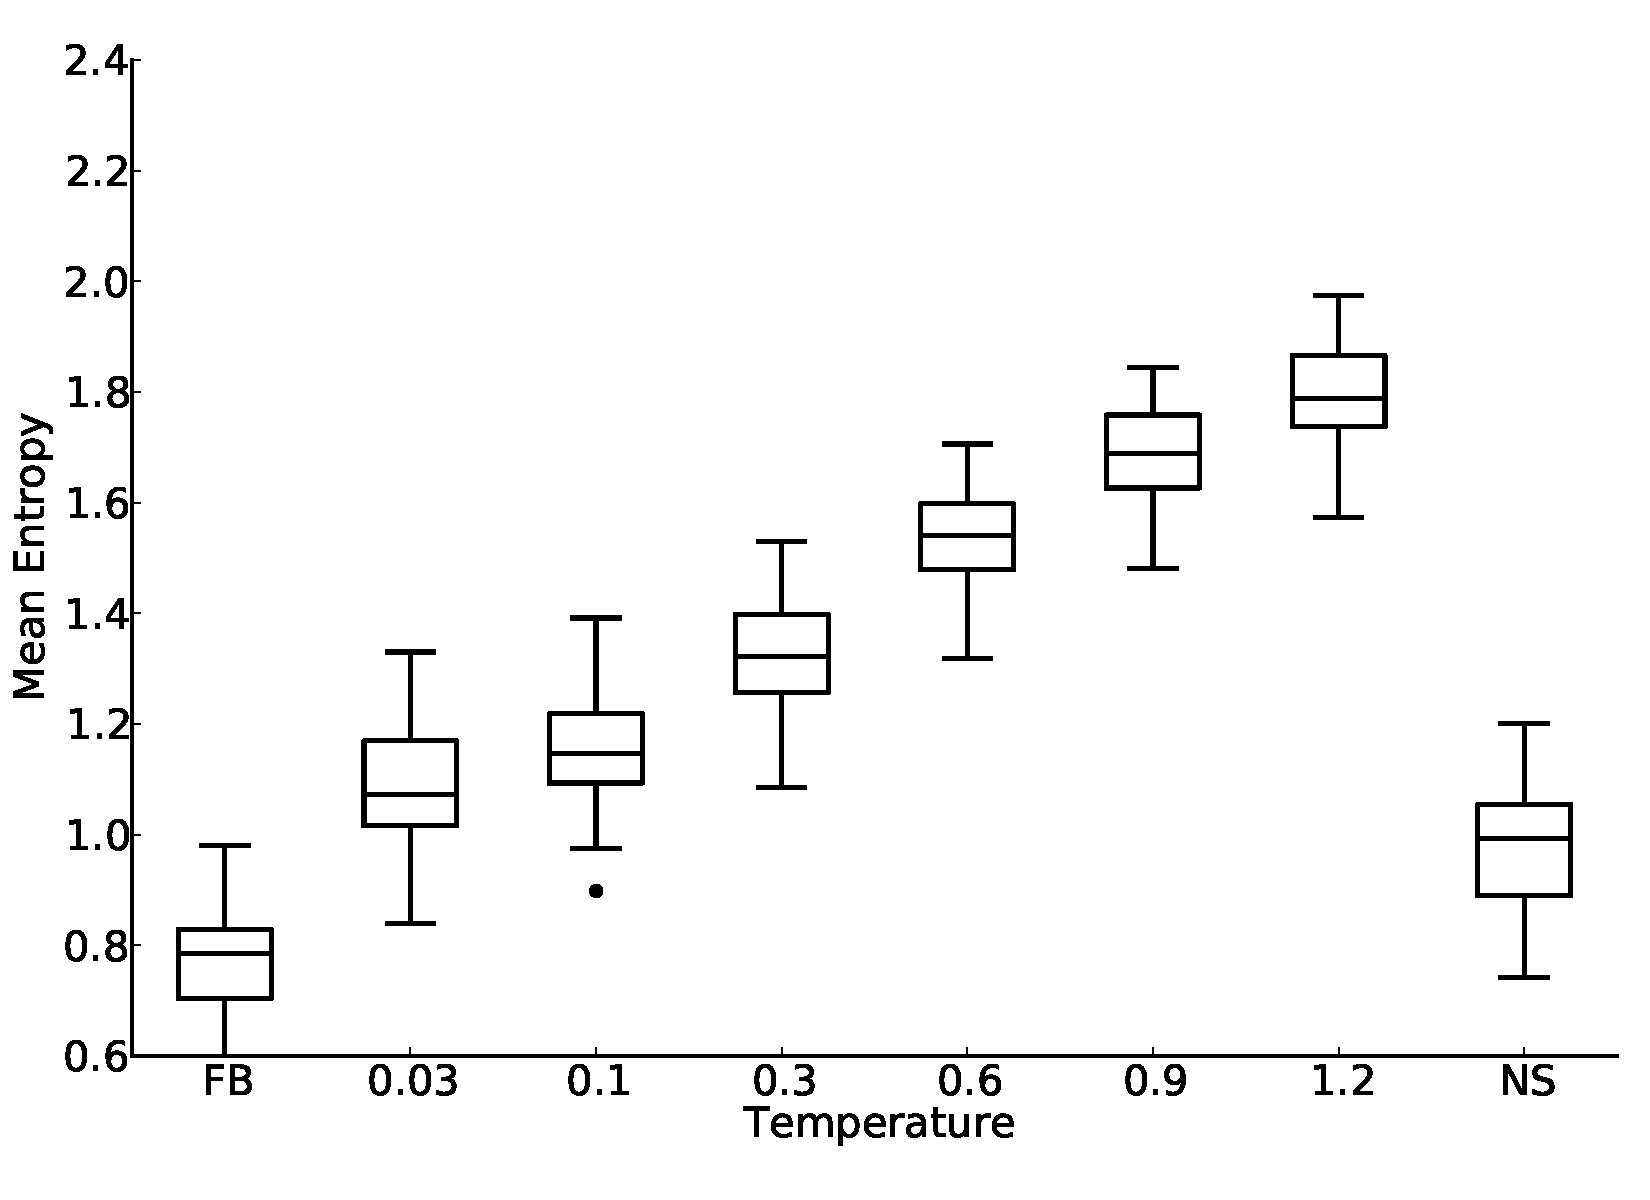
\includegraphics[width = 3in]{figures/Mean_Entropy_vs_Temp_Boxplot.pdf}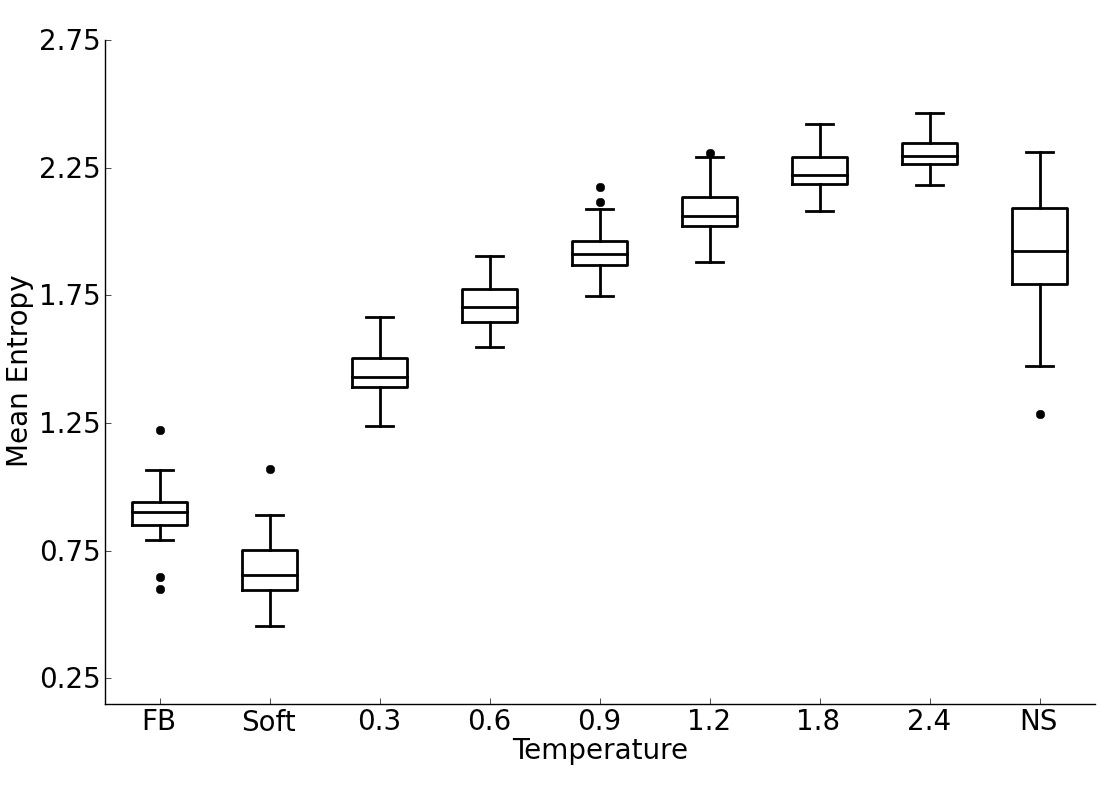
\includegraphics[width = 3in]{figures/Mean_Entropy_vs_Temp_Boxplot_Noah.pdf}}
\centerline{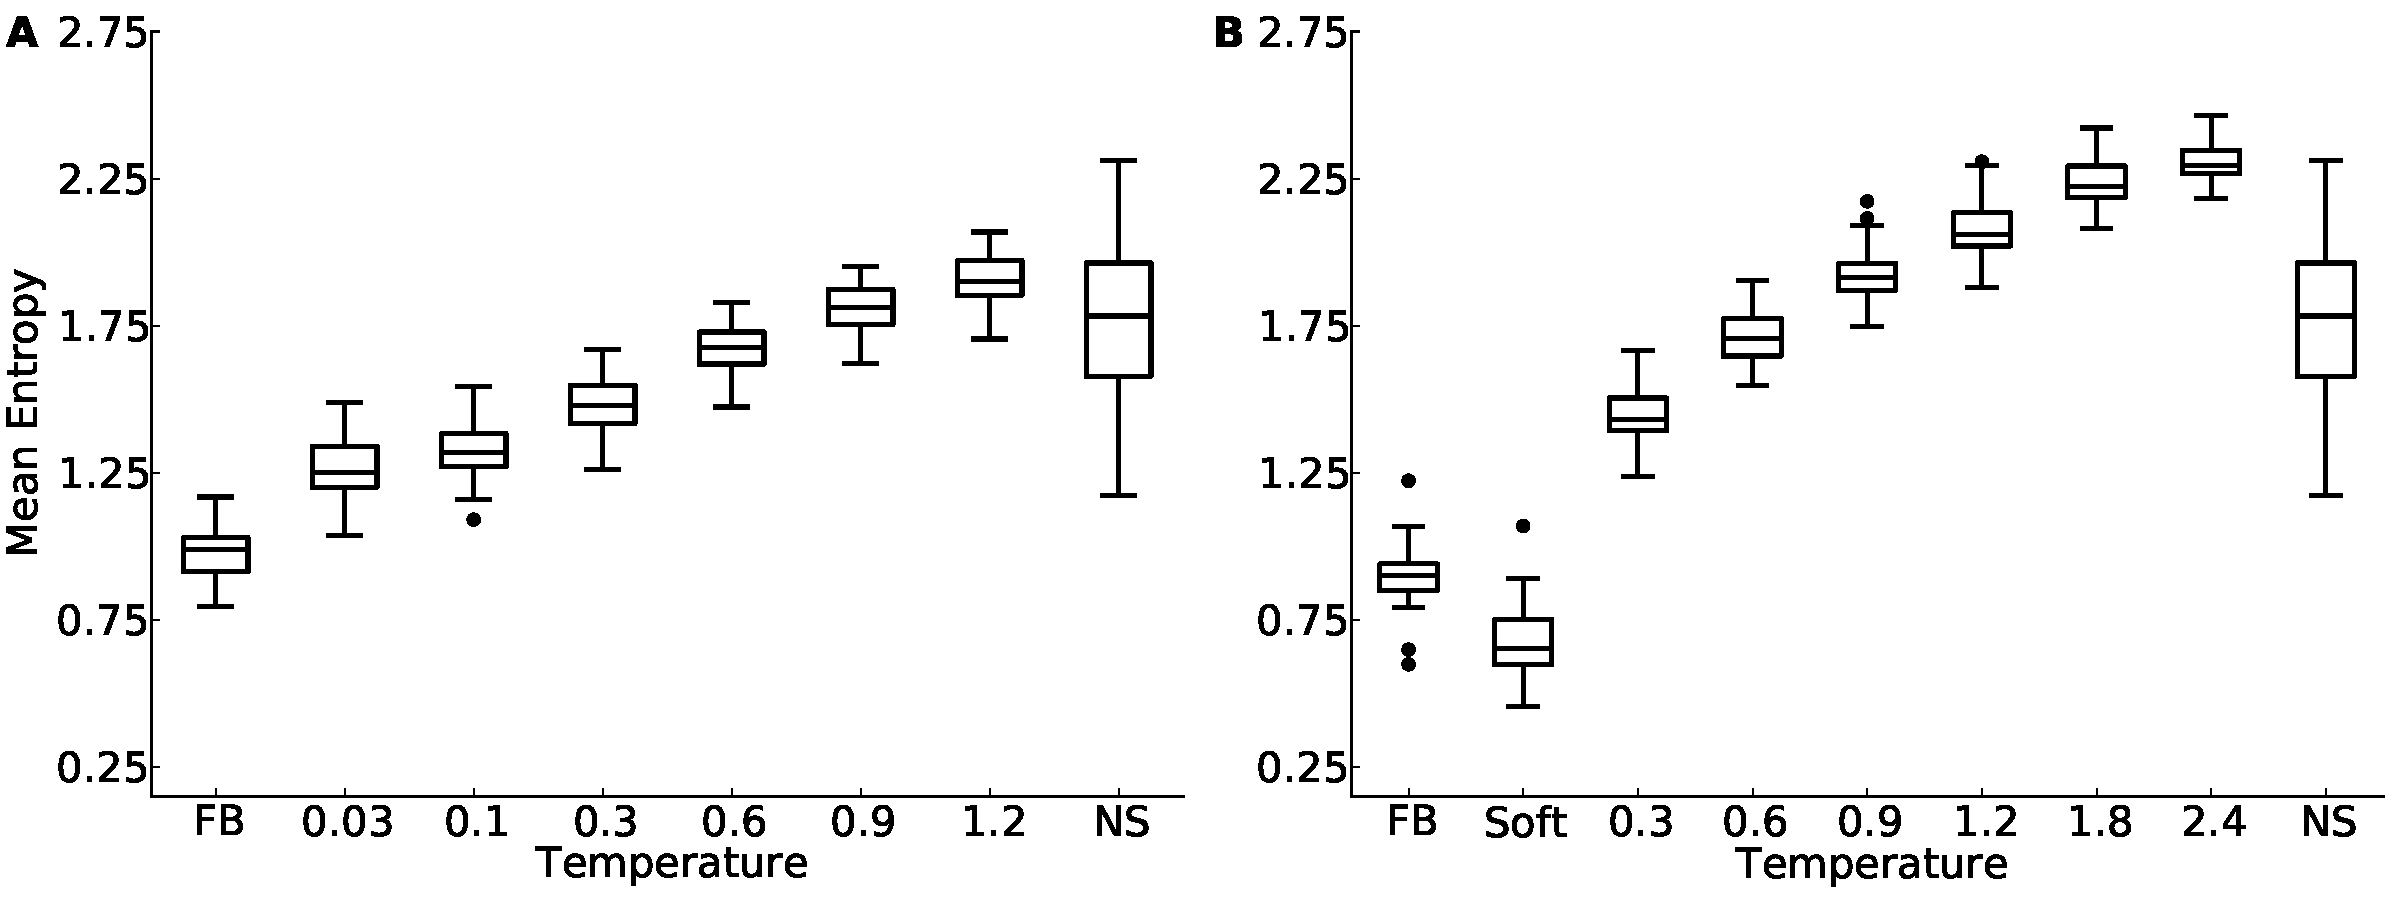
\includegraphics[width = 6in]{figures/Mean_Entropy_vs_Temp_Combo_Boxplot.pdf}} %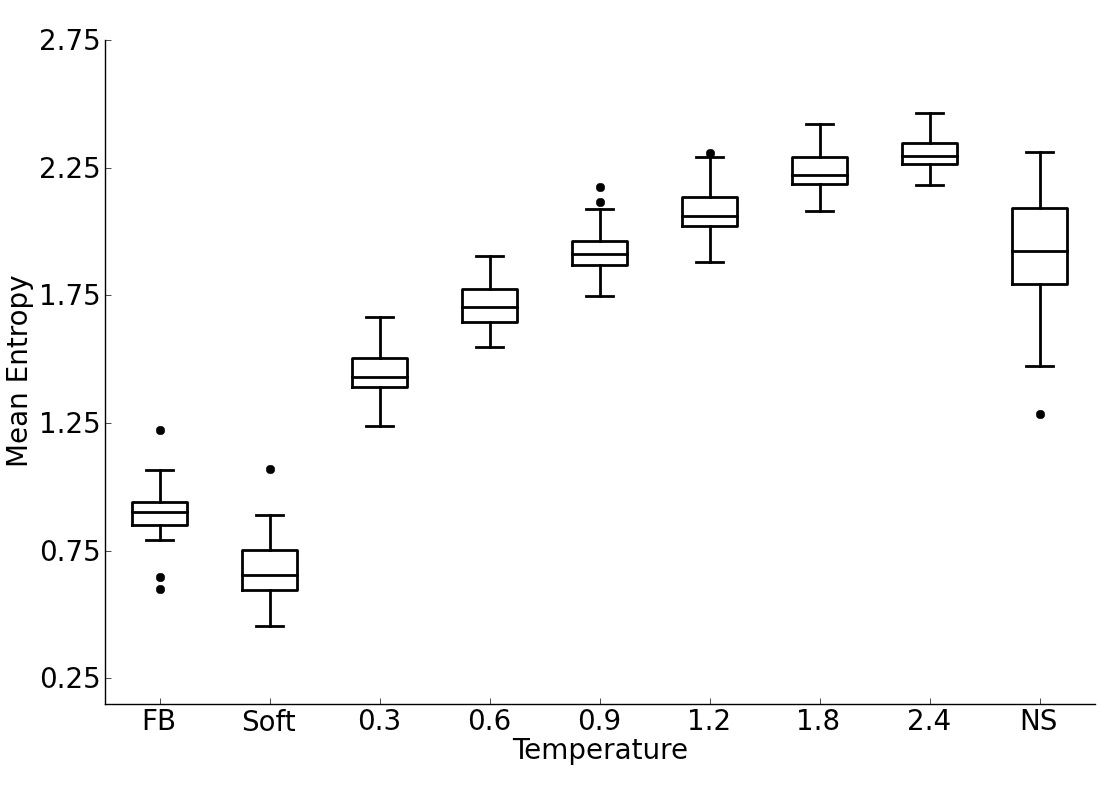
\includegraphics[width = 3in]{figures/Mean_Entropy_vs_Temp_Boxplot_Noah.pdf}}
\caption{Mean site entropy for designed and natural proteins. Each boxplot represents the distribution of mean site entropies within the respective dataset (left: yeast proteins; right: protein domains). ``FB'' refers to fixed-backbone design. Temperature values refer to the design temperature used during the Backrub design method. ``NS'' refers to natural sequences. ``Soft'' refers to the Soft design method. We find generally that more flexible backbones during desing allow for more site variability. Intermediate temperatures (0.6-0.9) produce site variabilities most similar to those seen in natural sequences. Overall, natural sequences in the protein-domains data set are more variable than are those in the yeast-proteins data set.}
\label{MeanEntropyComparison}
\end{figure}


\begin{figure}[H]
\centerline{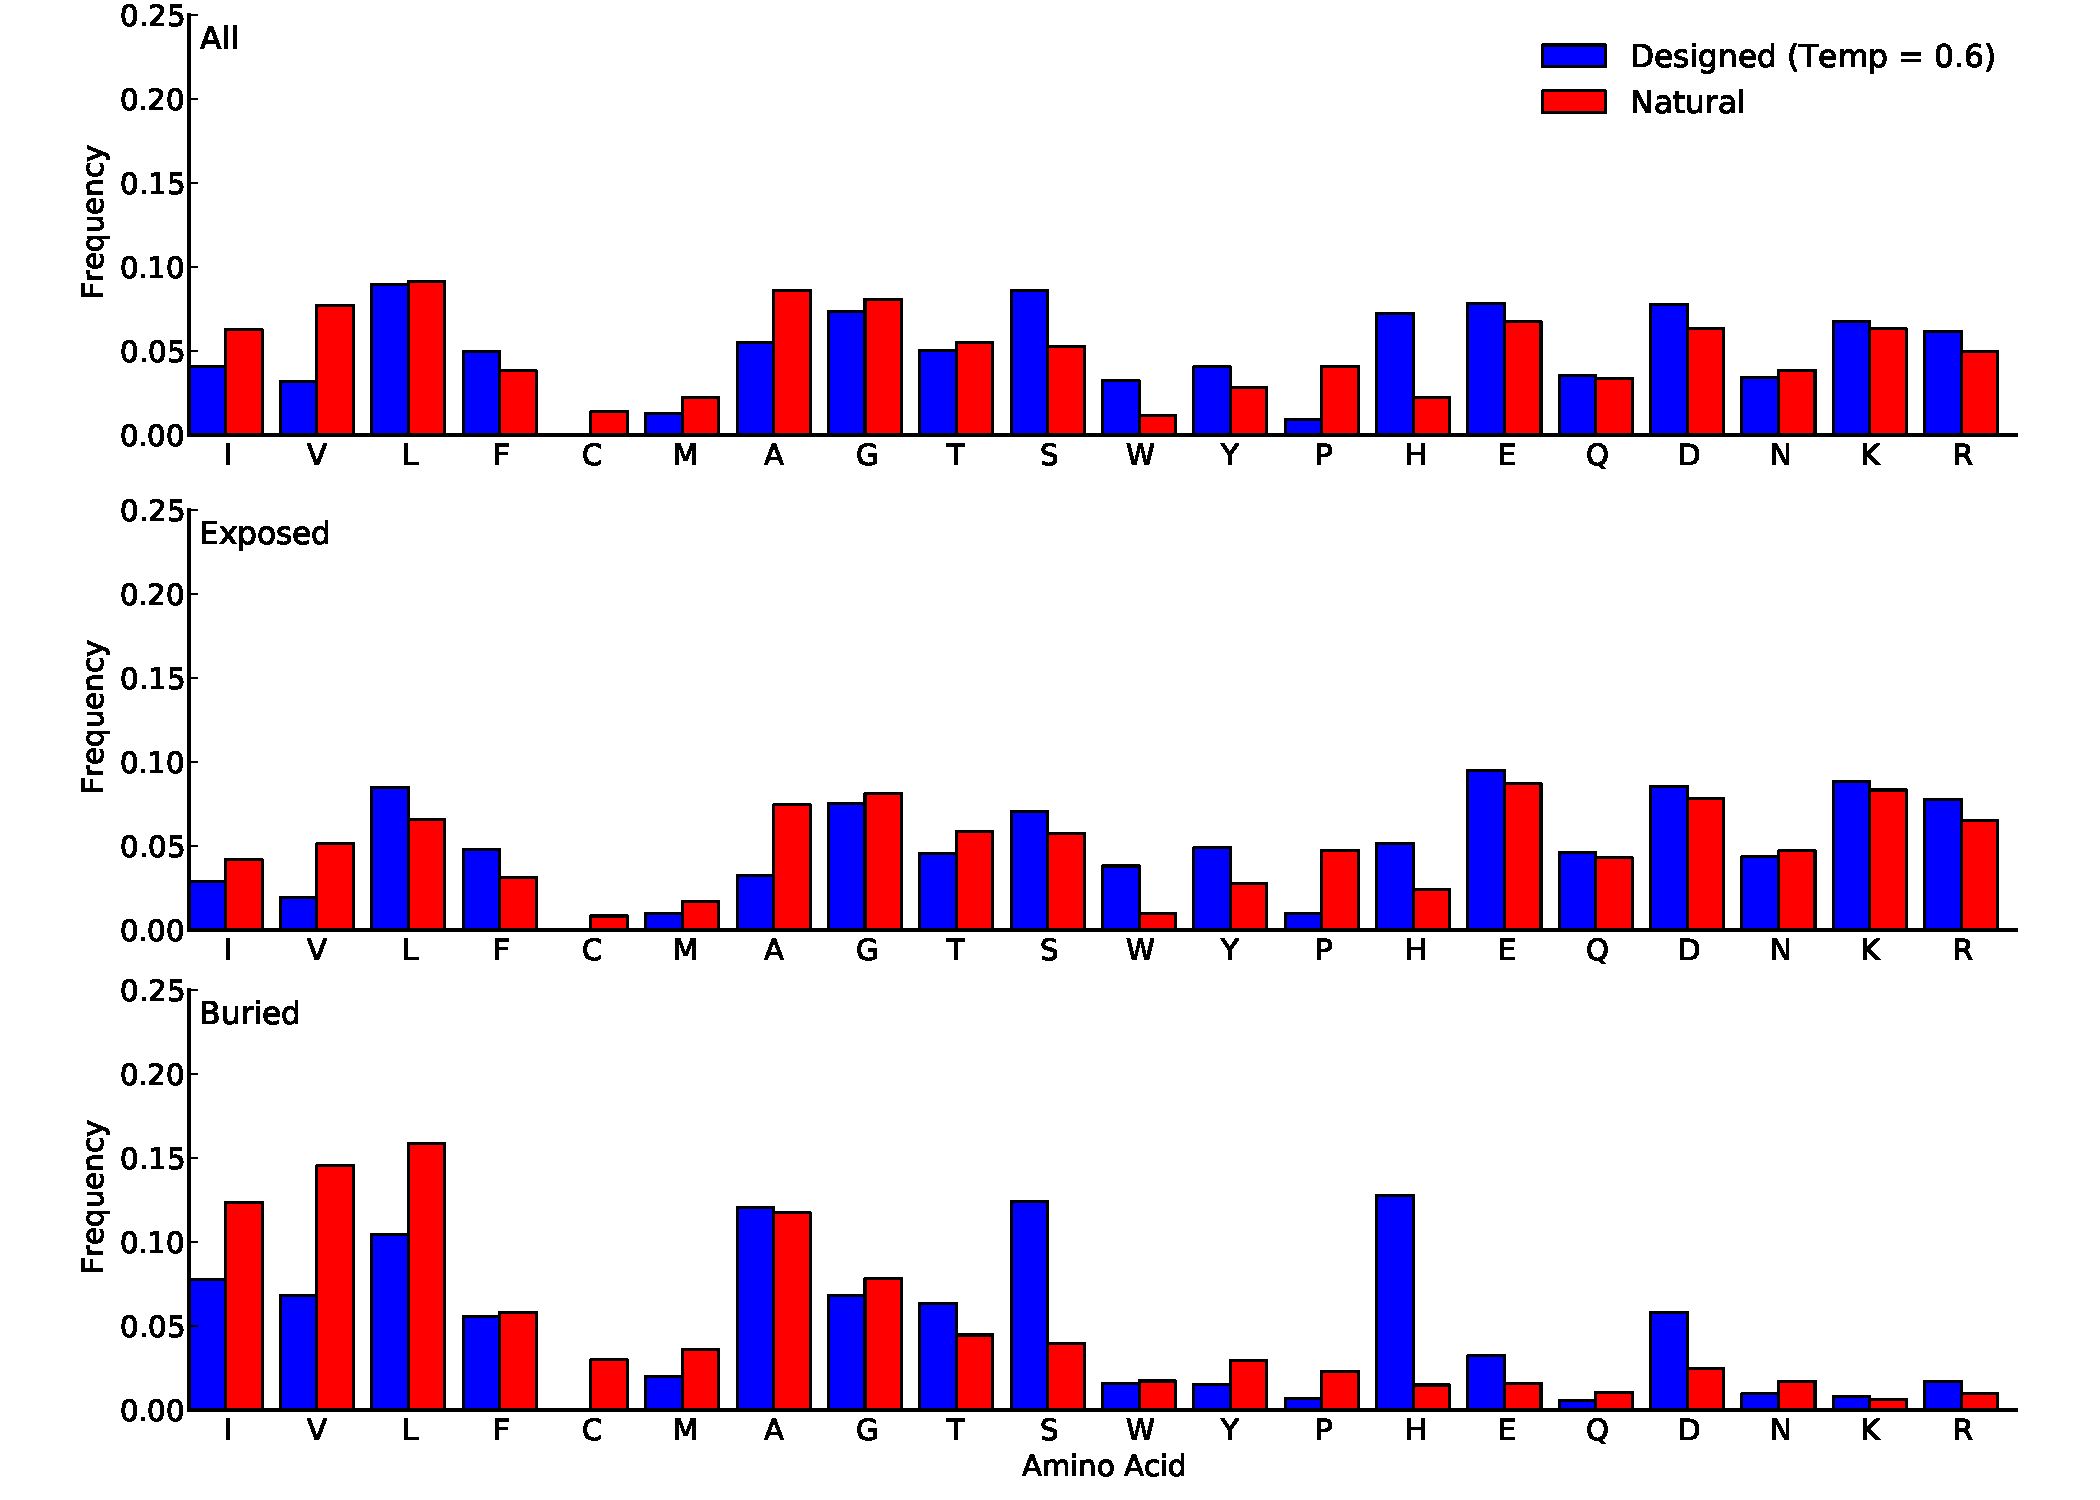
\includegraphics[width = 5in]{figures/Duncan_Freq_Combo_Plots_06.pdf}}
\caption{Amino-acid frequencies in designed and natural proteins. Frequencies were calculated over all sites in all proteins belonging to the yeast-proteins data set. For designed proteins, only flexible-backbone designs with design temperature 0.6 were considered. Top: overall frequencies. Middle: frequencies at exposed sites (defined as sites with $\text{RSA}>0.05$). Bottom: frequencies at buried sites (defined as sites with $\text{RSA}\leq0.05$).}
\label{AAFreqsYeastProteins}
\end{figure}


\begin{figure}[H]
\centerline{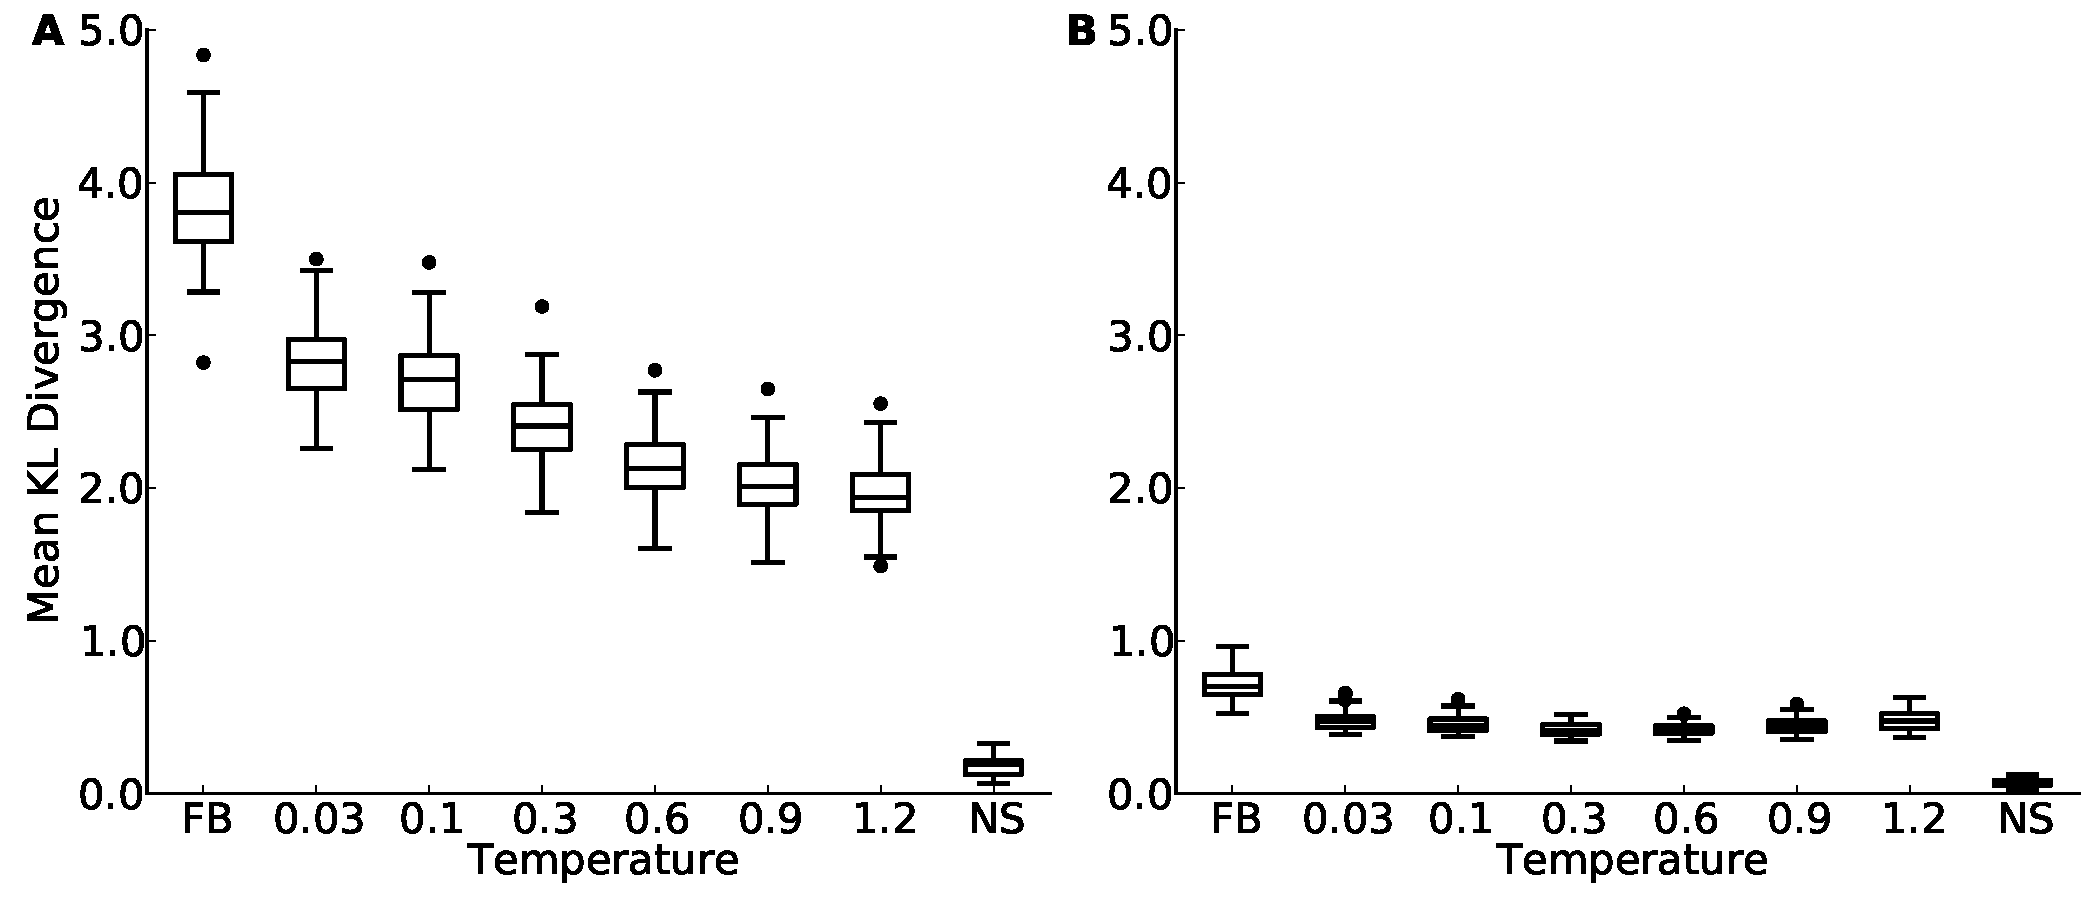
\includegraphics[width = 6in]{figures/Mean_KL_vs_Temp_Boxplot.pdf}}
\caption{Mean Kullback-Leibler (KL) divergence for designed and natural proteins, shown for the yeast-proteins data set. A higher KL divergence indicates that the amino-acid distributions at sites in designed proteins are less similar to the corresponding distributions in the natural proteins. ``FB'' refers to fixed backbone design, and ``NS'' refers to the control case where natural sequences are compared to themselves. (A) KL divergence calculated from the relative frequencies of the 20 amino acids. (B) KL divergence calculated from rank-ordered frequency distributions. The most common amino aicd in the reference distribution is compared to the most common amino acid in the focal distribution, the same is done for the second-most common amino acid, and so on, irrespective of the type of amino acids.}
\label{AADisFig1}
\end{figure}


\begin{figure}[H]
\centerline{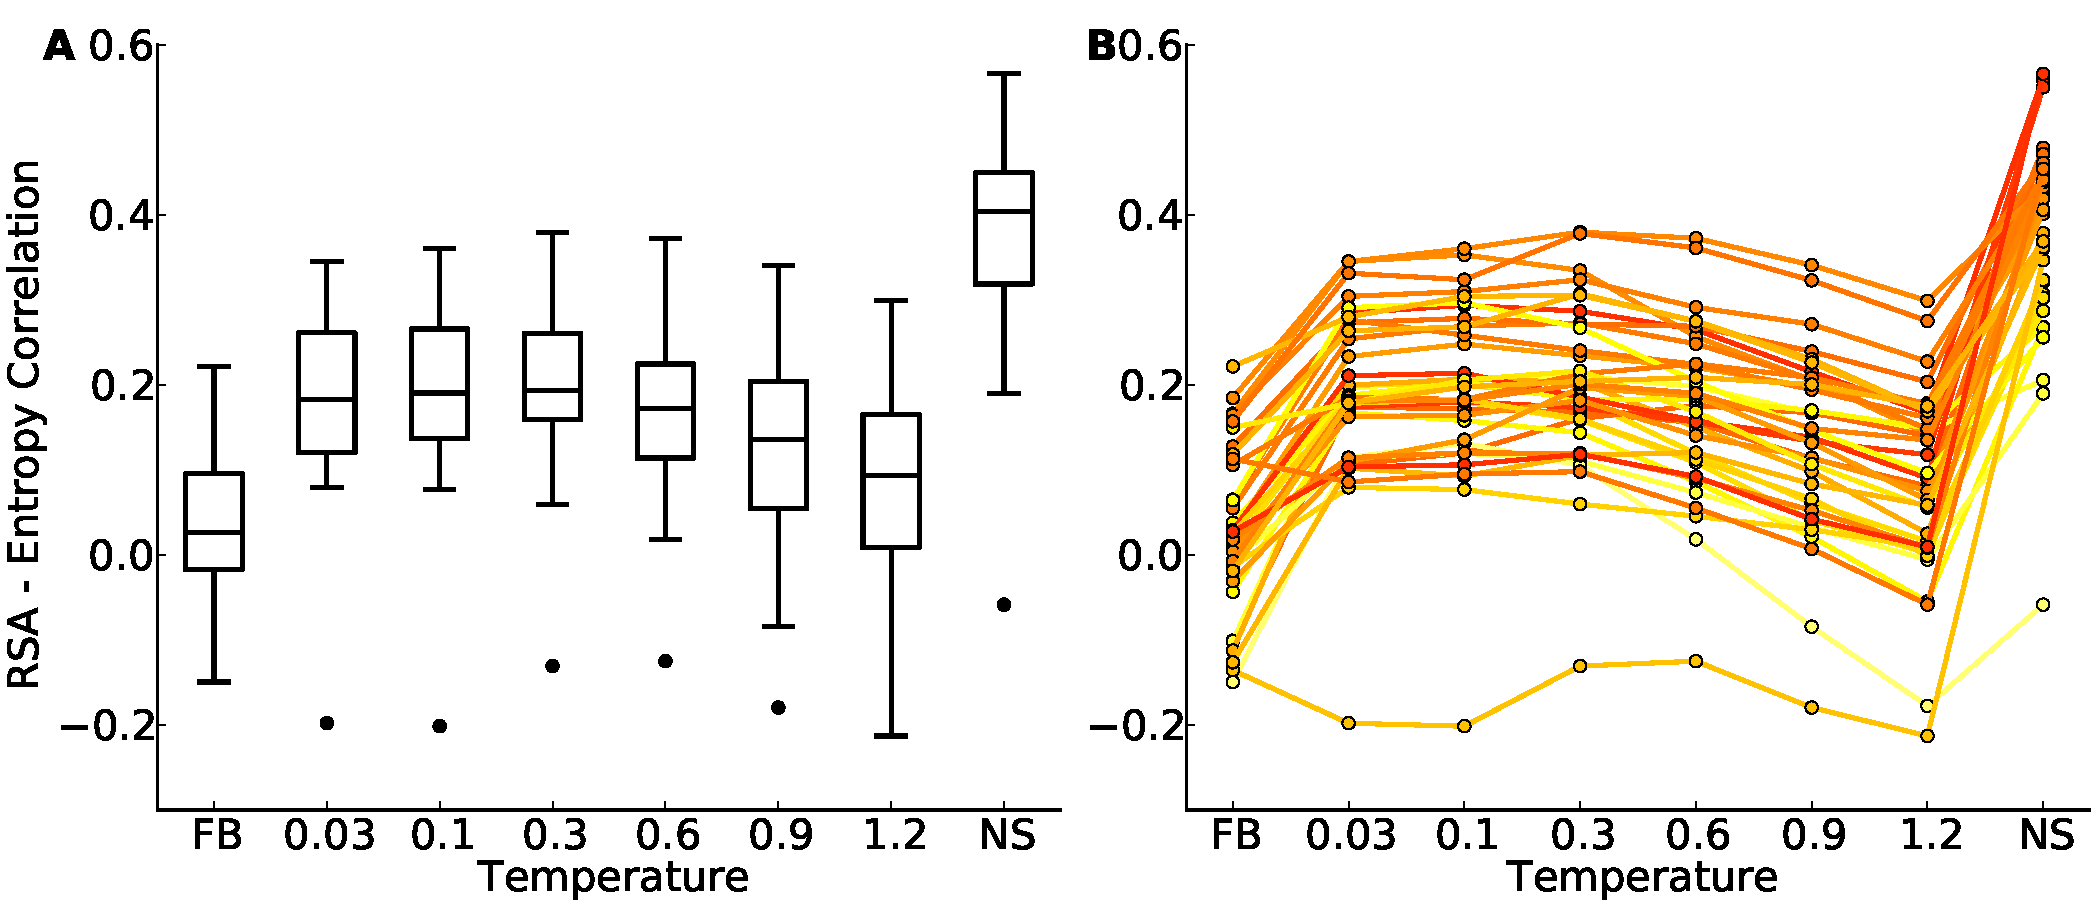
\includegraphics[width = 6in]{figures/Cor_Mean_Entropy_RSA_Combination_Plot.pdf}}
\caption{Distributions of correlation coefficients between site entropy and RSA, for the yeast-proteins data set. ``FB'' indicates fixed-backbone design, and ``NS'' indicates natural sequences. (A) Distributions represented as boxplots. (B) Correlation coefficients for individual proteins. Lines connect identical structures in the different design conditions. The color shading represents the strength of the correlation for the natural sequence alignment. In general, natural proteins display a stronger correlation between site entropy and RSA than designed proteins.}
\label{Correlation_figure}
\end{figure}


\begin{figure}[H]
%\centerline{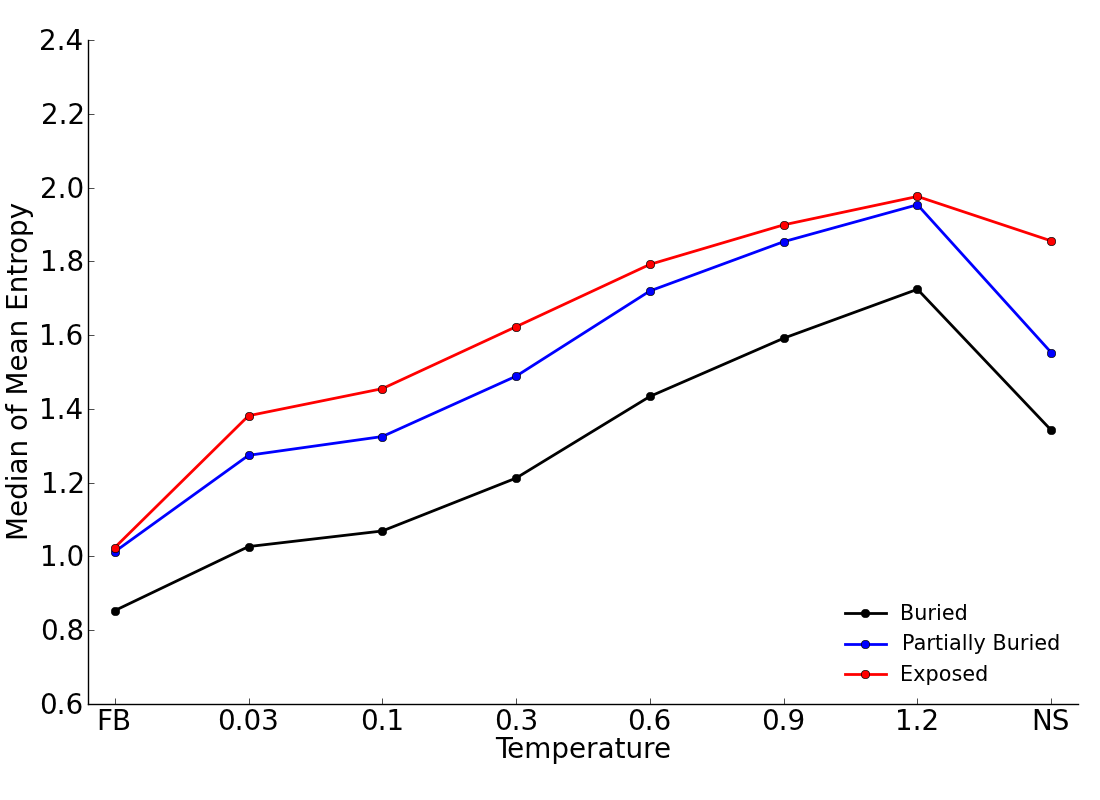
\includegraphics[width = 3in]{figures/Mean_Entropy_Position_Lineplot.pdf}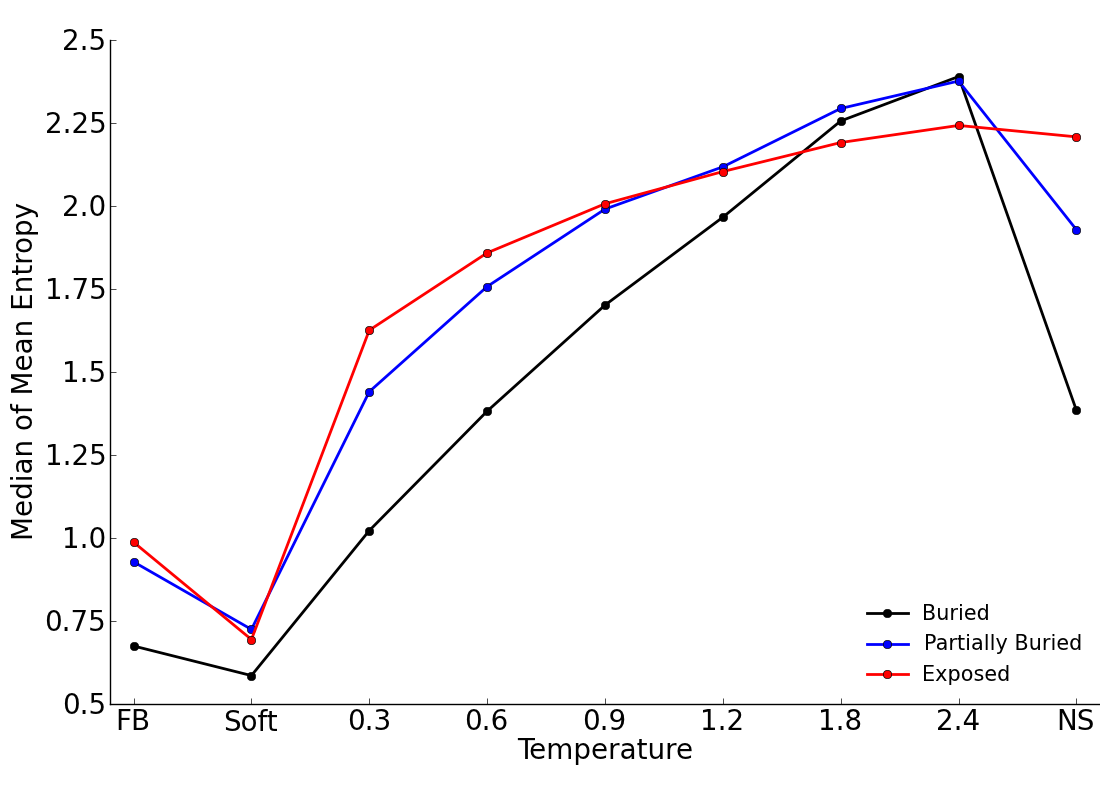
\includegraphics[width = 3in]{figures/Mean_Entropy_Position_Lineplot_Noah.pdf}}
\centerline{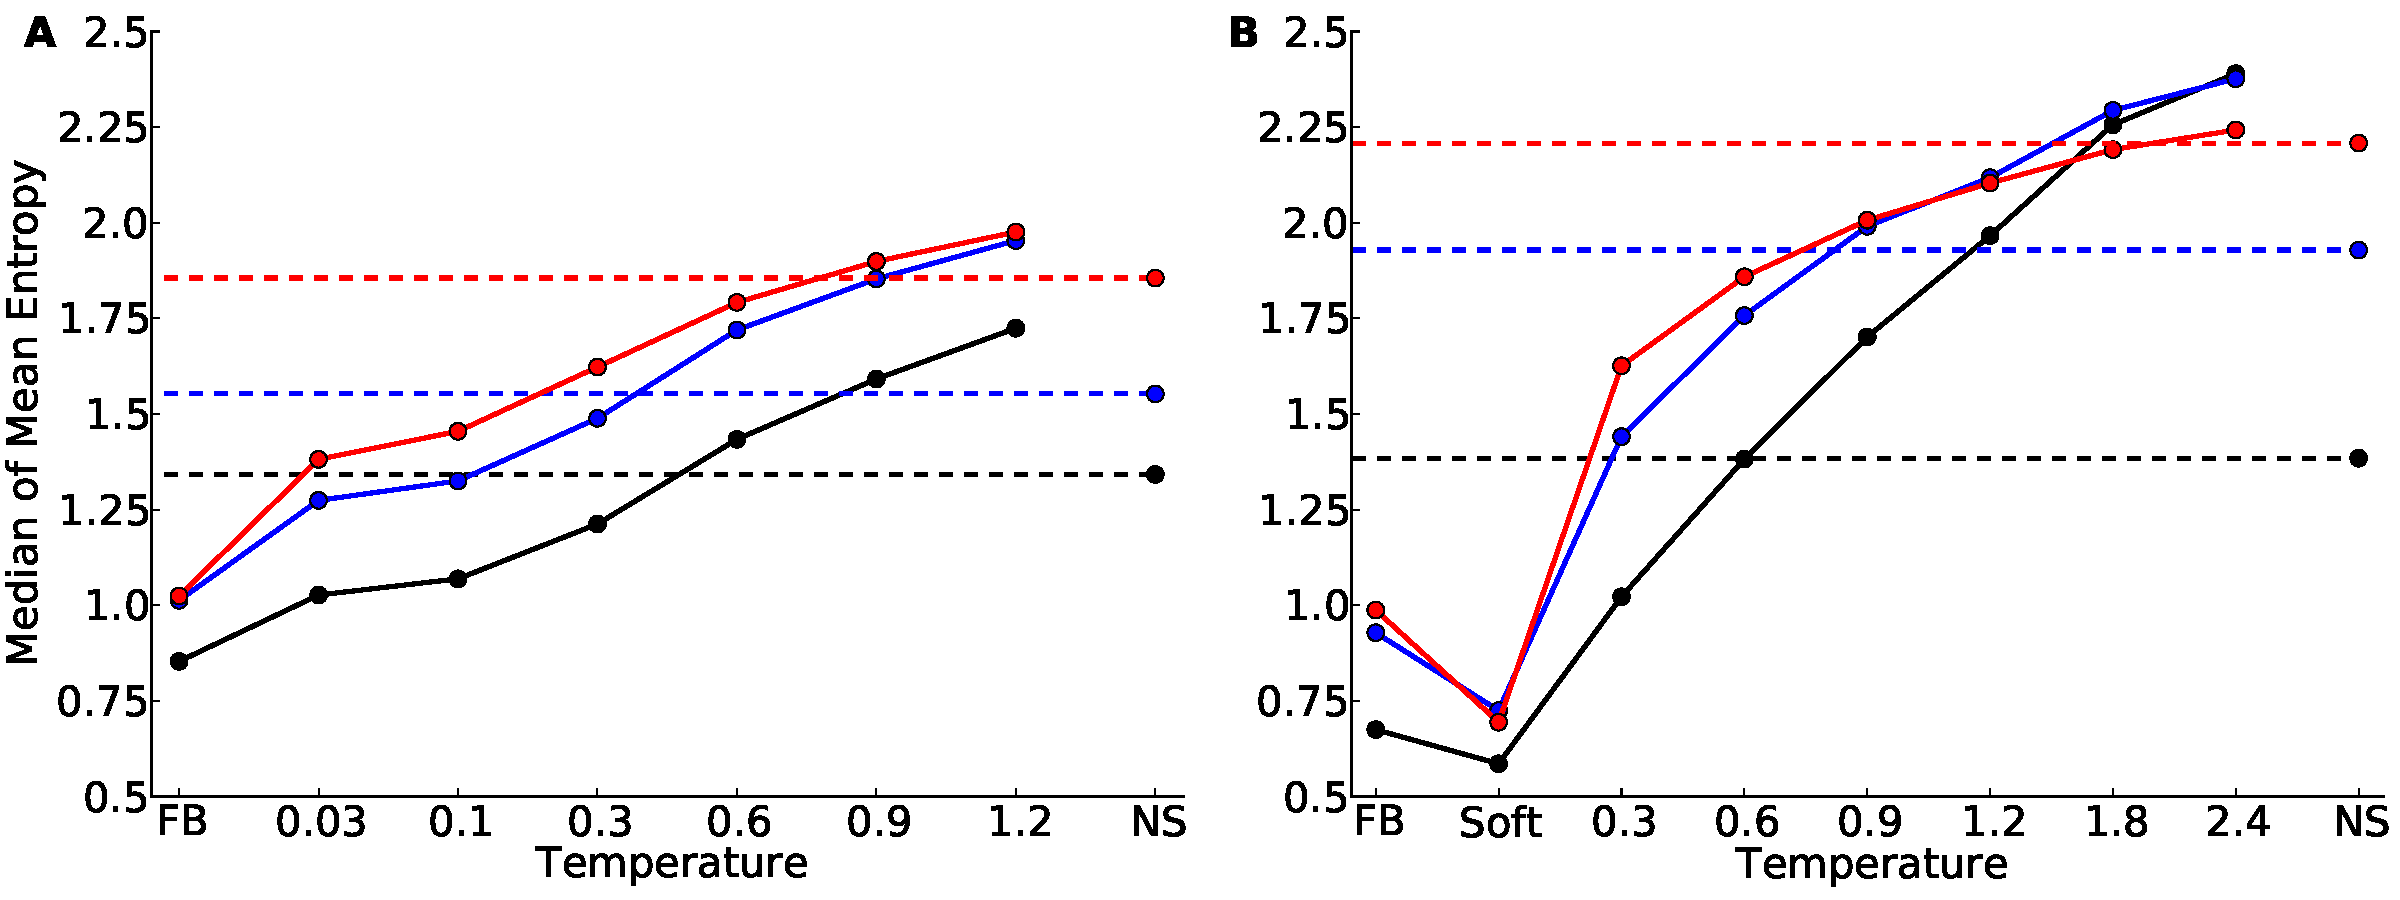
\includegraphics[width = 6in]{figures/Mean_Entropy_Position_Lineplot_Combo.pdf}}
\caption{Median of the distribution of mean sequence entropies for designed and natural sequences, calculated separately for buried, partially buried, and exposed residues (left: yeast proteins; right: protein domains). We defined buried sites as those with $\text{RSA}\leq 0.05$, partially buried as those with $0.05<\text{RSA}\leq0.25$, and exposed as those with $\text{RSA}>0.25$. Connecting lines are meant as a guide to the eye. Note the difference in the $x$-axis scales between the two graphs.}
\label{Mean_Entropy_Surface_Core}
\end{figure}


\begin{figure}[H]
%\centerline{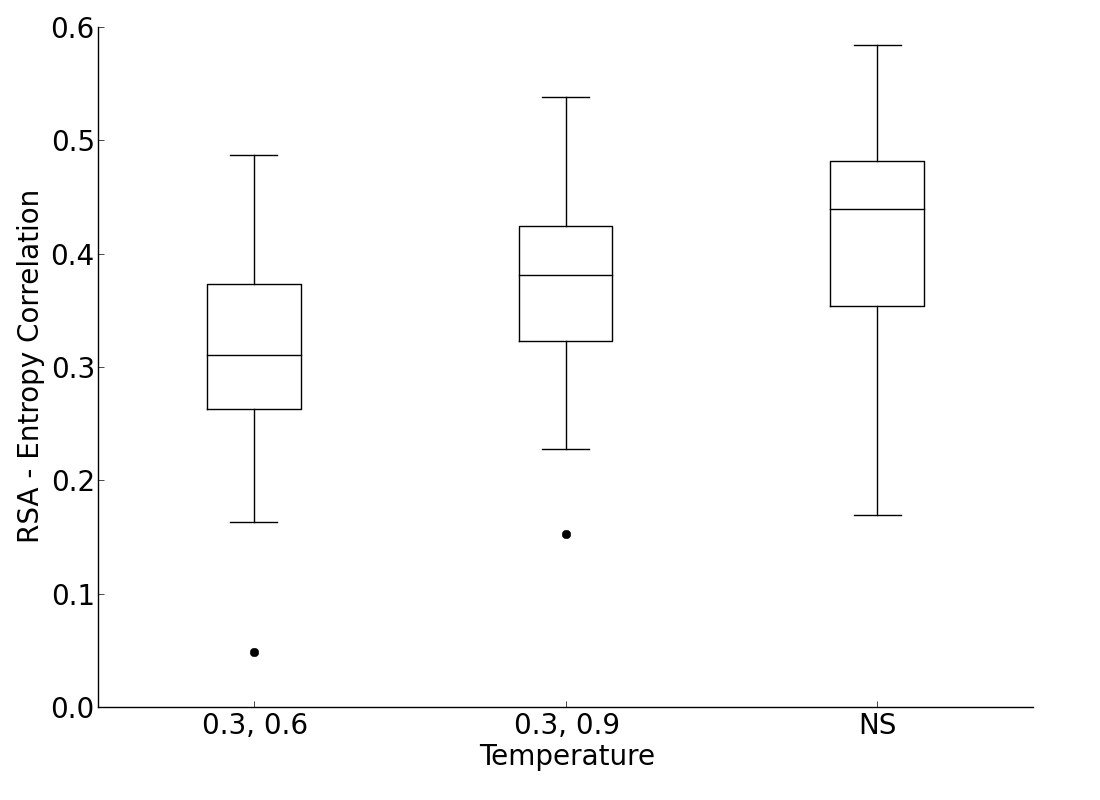
\includegraphics[width = 3in]{figures/Duncan_Mixed_Temp_Correlation_Plot.pdf}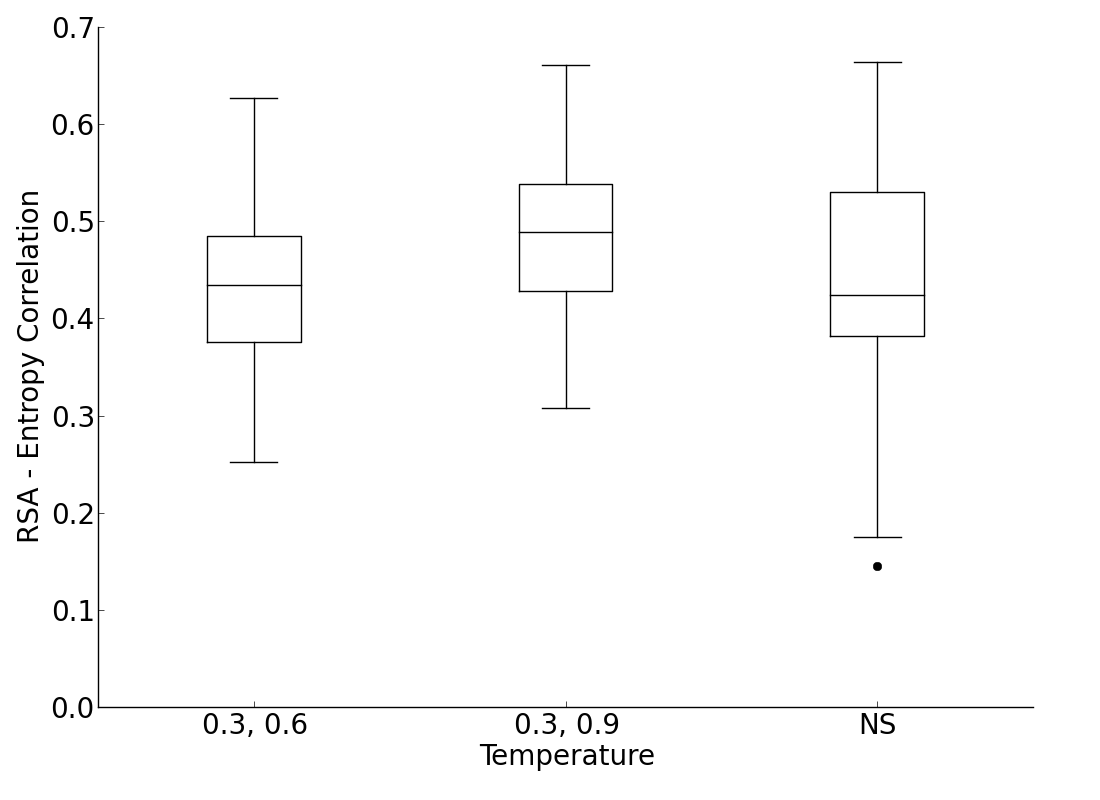
\includegraphics[width = 3in]{figures/Noah_Mixed_Temp_Correlation_Plot.pdf}}
\centerline{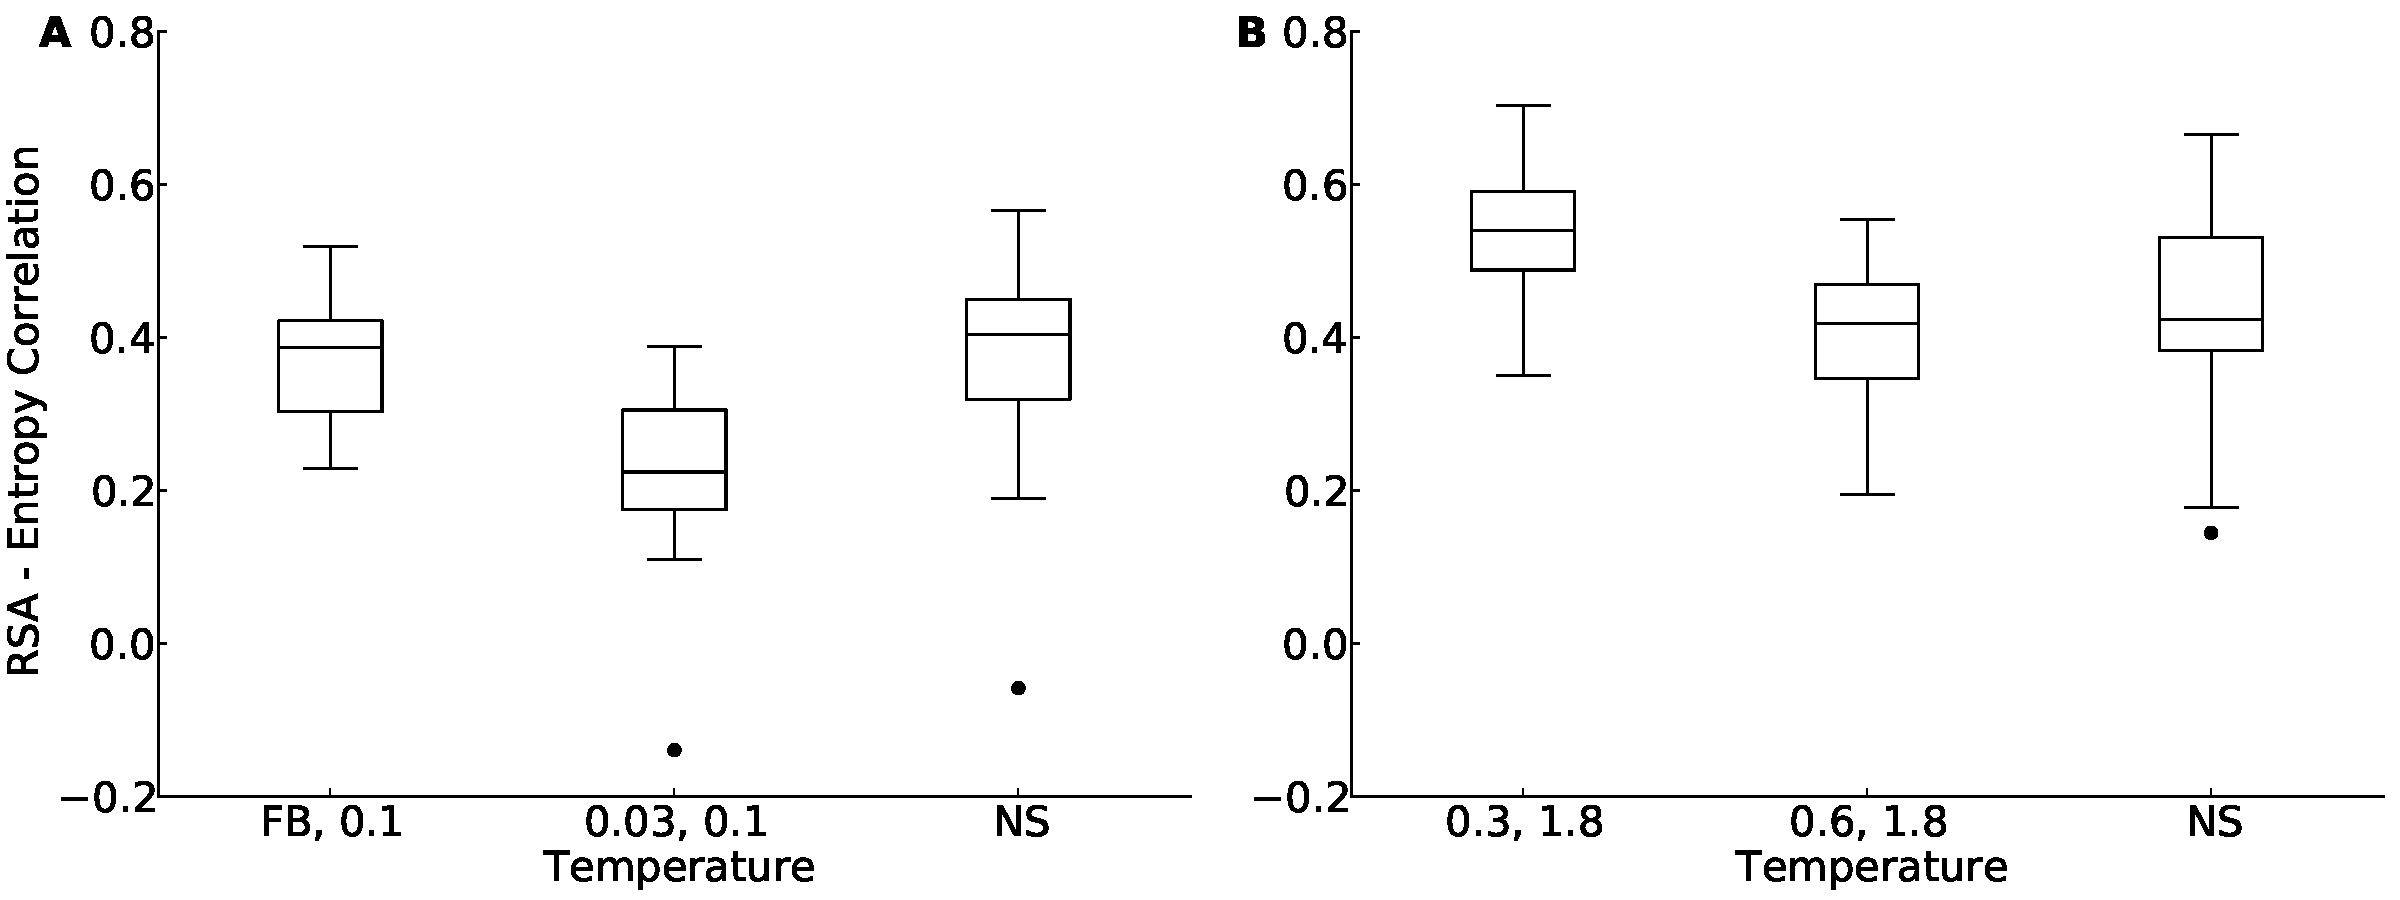
\includegraphics[width = 6in]{figures/Combo_Mixed_Temp_Correlation_Plot.pdf}}
\caption{Distribution of correlation coefficients between RSA and site entropy for hybrid designs and for natural proteins. For the hybrid designs, buried sites were taken from sequences designed at one temperature, and partially buried and exposed sites were taken from sequences designed at a different temperature. For the hybrid designs, the correlation coefficients were similar to those of natural sequences ({\color{red}paired $t$ test, $P=\dots$ and $P=\dots$ [yeast proteins], $P=\dots$ and $P=\dots$ [protein domains]}). {\color{red}\emph{ Can you make a version of this figure that looks like Fig. 4B? And finally, we'll have to talk about $x$ axis labeling.}}}
\label{Mixed_RSA_Entropy}
\end{figure}


\cleardoublepage

\section{Supporting Figures}

\centerline{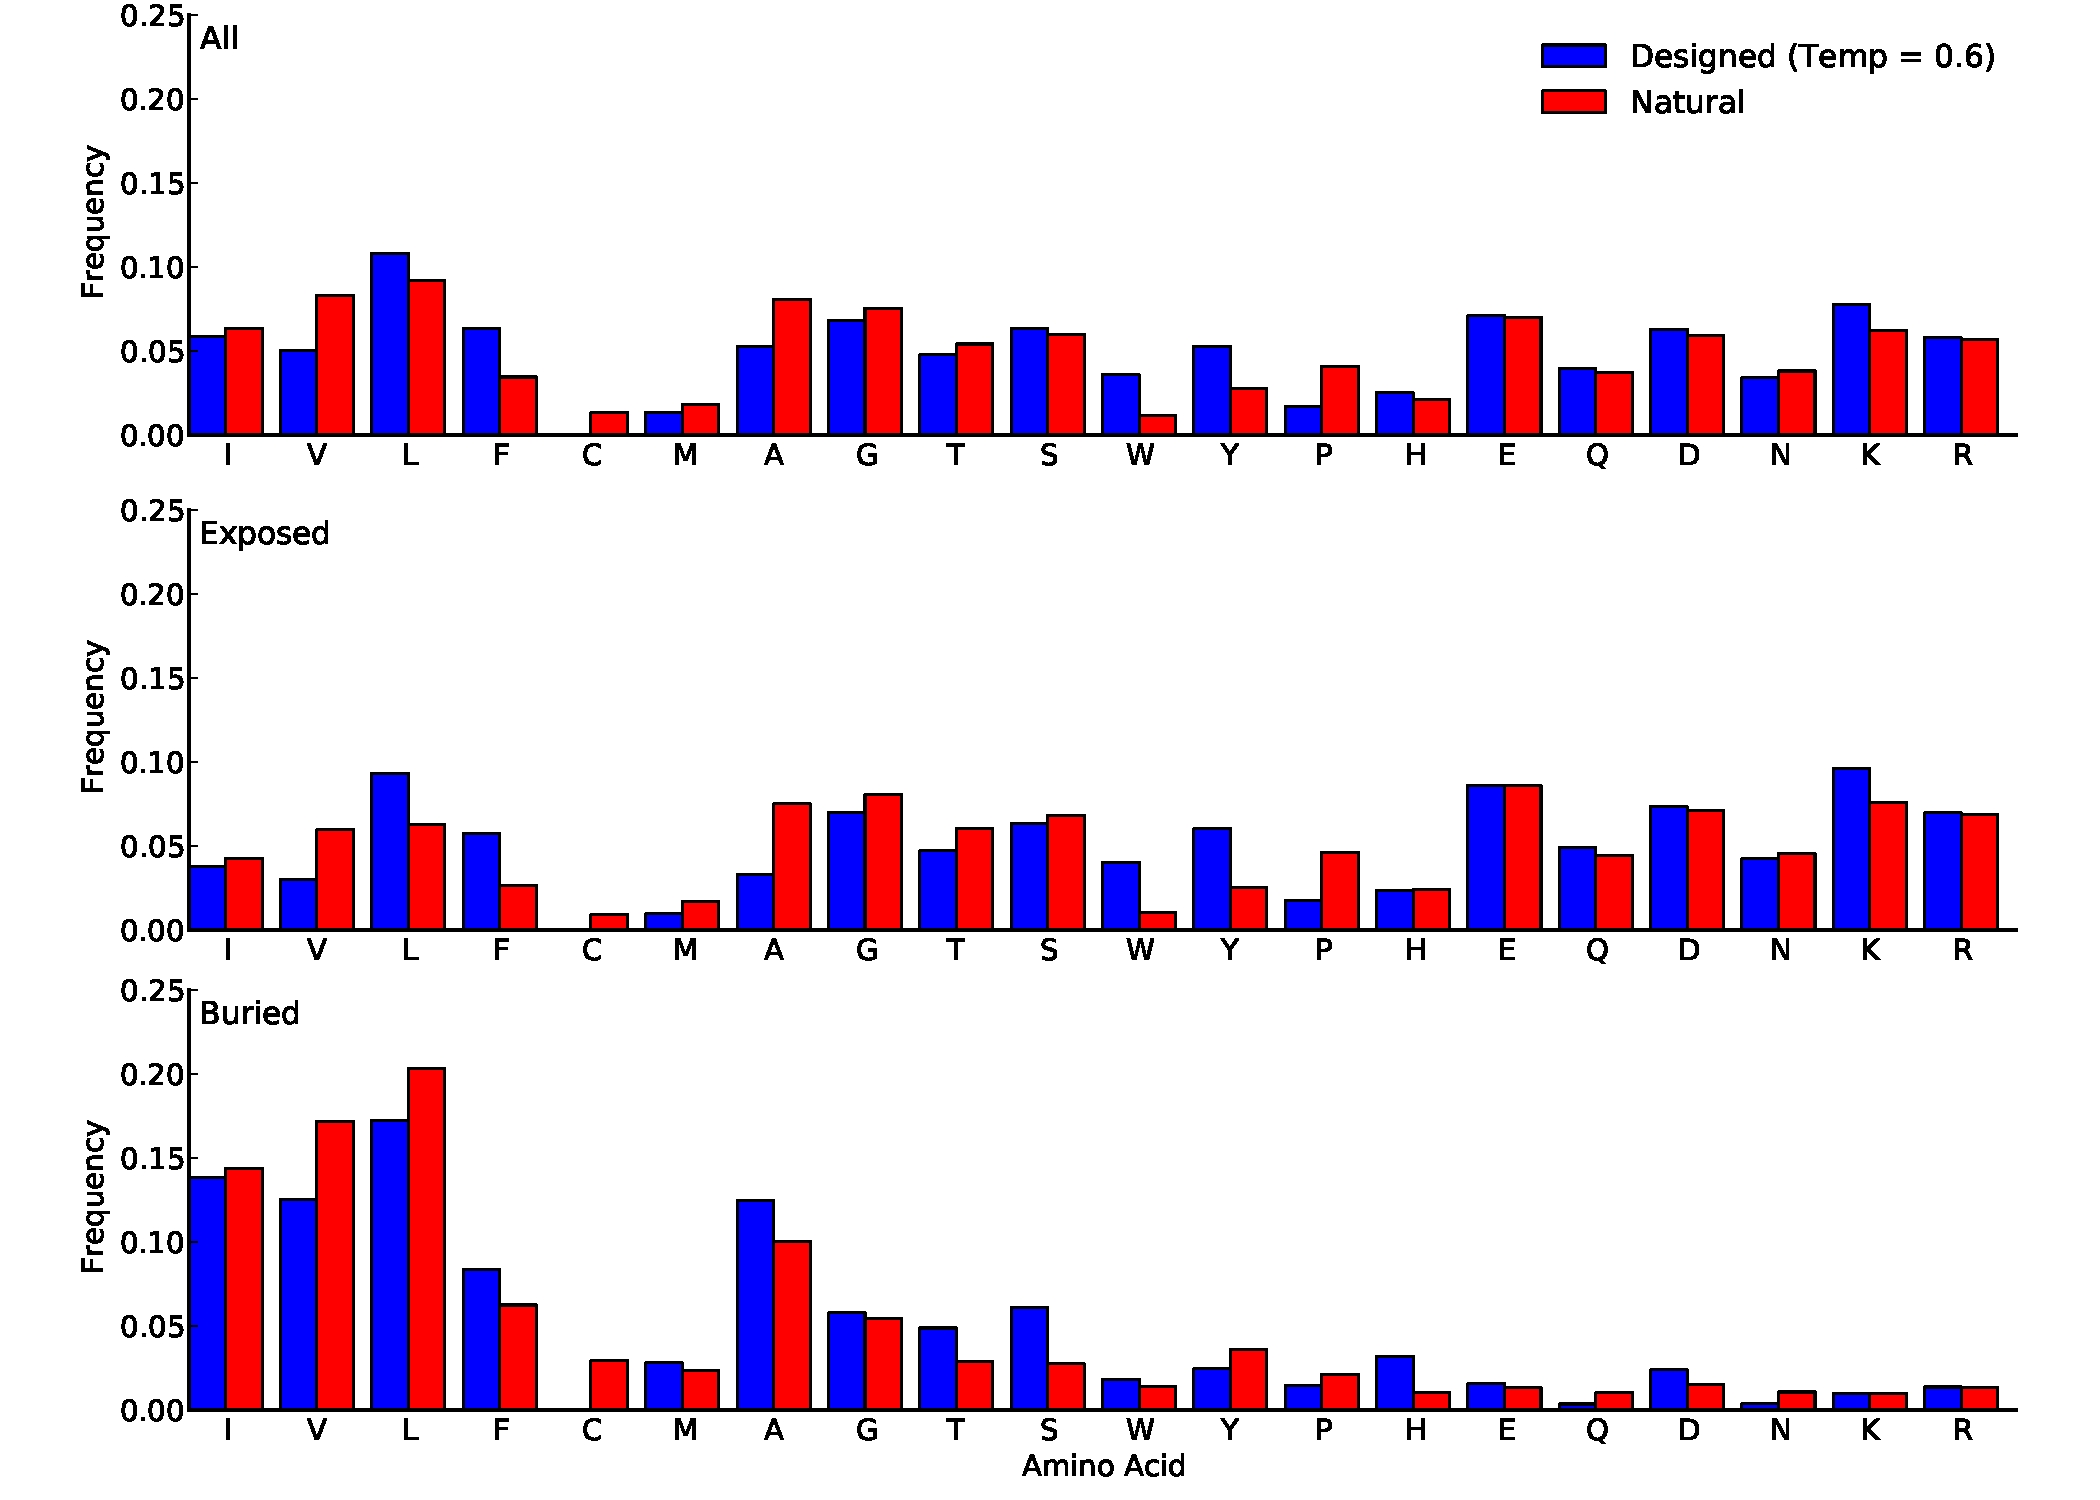
\includegraphics[width = 5in]{figures/Noah_Freq_Combo_Plots_06.pdf}}

\noindent Figure S1. Amino-acid frequencies in designed and natural proteins. Frequencies were calculated over all sites in all proteins belonging to the protein-domains data set. For designed proteins, only flexible-backbone designs with design temperature 0.6 were considered. Top: overall frequencies. Middle: frequencies at exposed sites (defined as sites with $\text{RSA}>0.05$). Bottom: frequencies at buried sites (defined as sites with $\text{RSA}\leq0.05$).

\customlabel{AAFreqsProteinDomains}{S1}

\newpage

\centerline{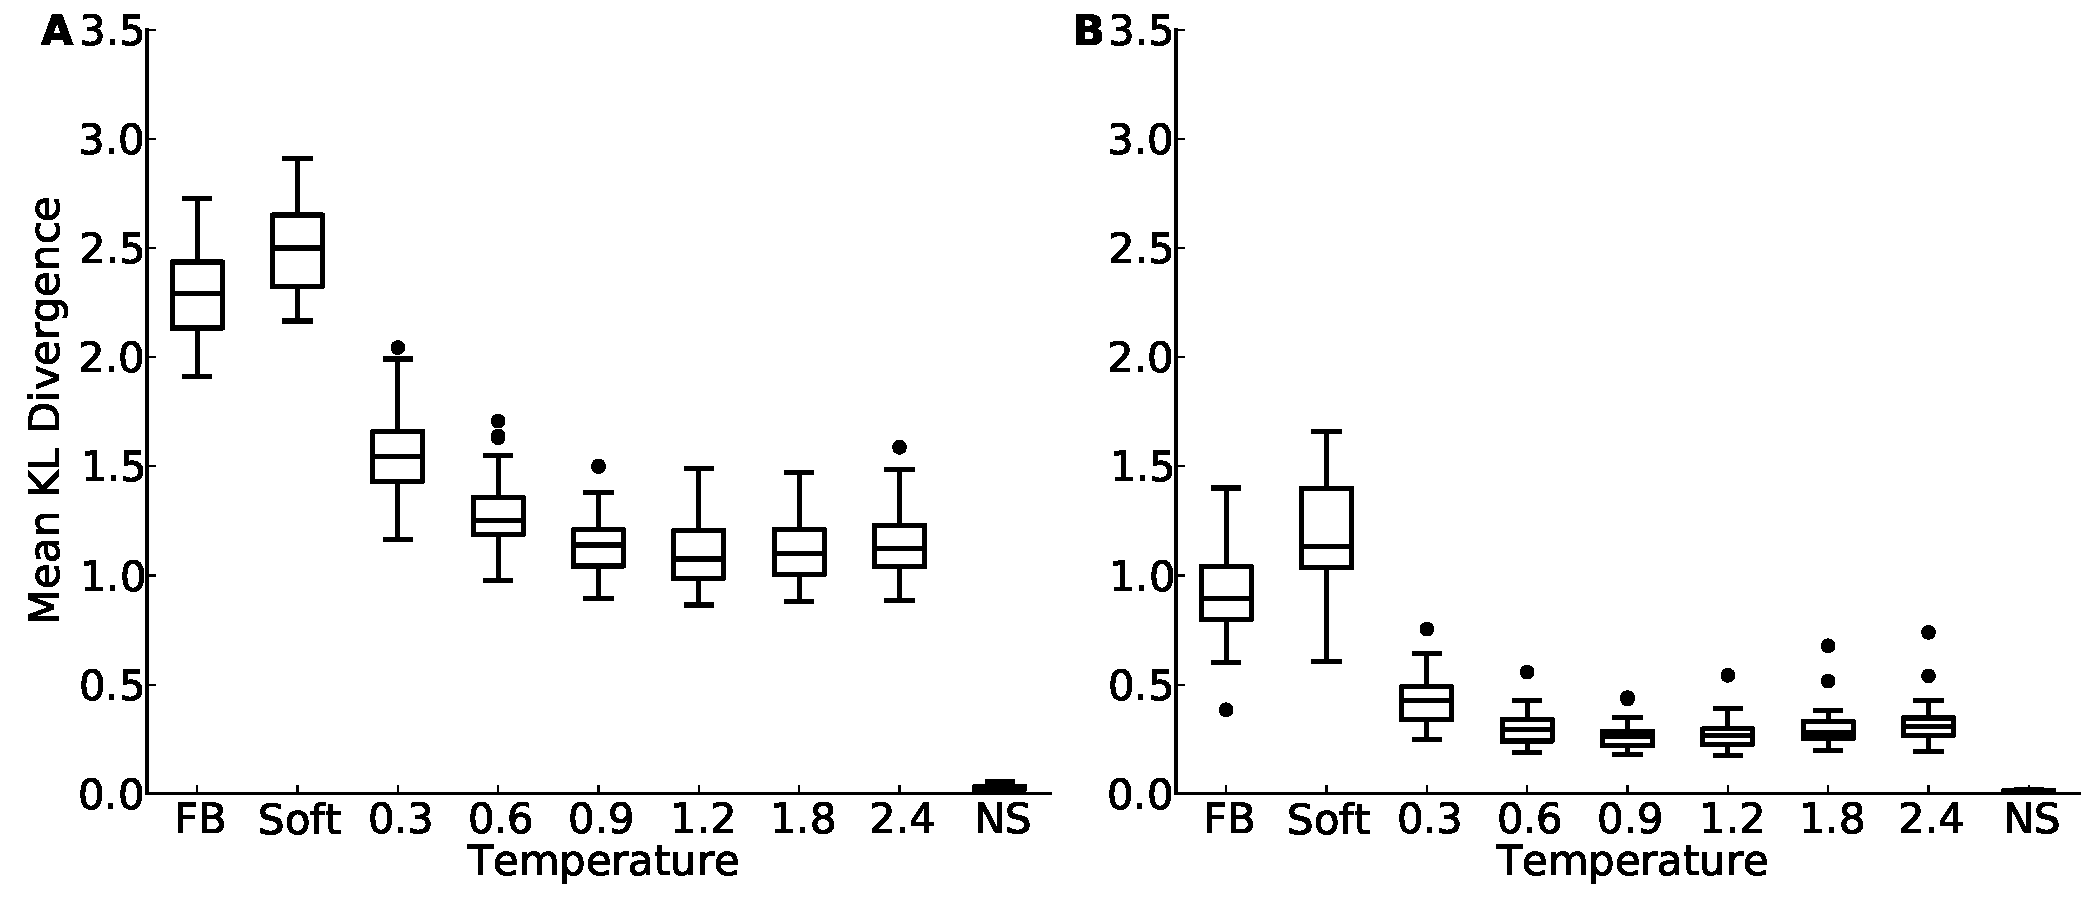
\includegraphics[width = 6in]{figures/Mean_KL_vs_Temp_Boxplot_Noah.pdf}}
\noindent Figure S2. Mean Kullback-Leibler (KL) divergence for designed and natural proteins, shown for the yeast-proteins data set. A higher KL divergence indicates that the amino-acid distributions at sites in designed proteins are less similar to the corresponding distributions in the natural proteins. ``FB'' refers to fixed backbone design, and ``NS'' refers to the control case where natural sequences are compared to themselves. (A) KL divergence calculated from the relative frequencies of the 20 amino acids. (B) KL divergence calculated from rank-ordered frequency distributions. The most common amino aicd in the reference distribution is compared to the most common amino acid in the focal distribution, the same is done for the second-most common amino acid, and so on, irrespective of the type of amino acids.

\customlabel{NoahAADisFig1}{S2}

\newpage


\centerline{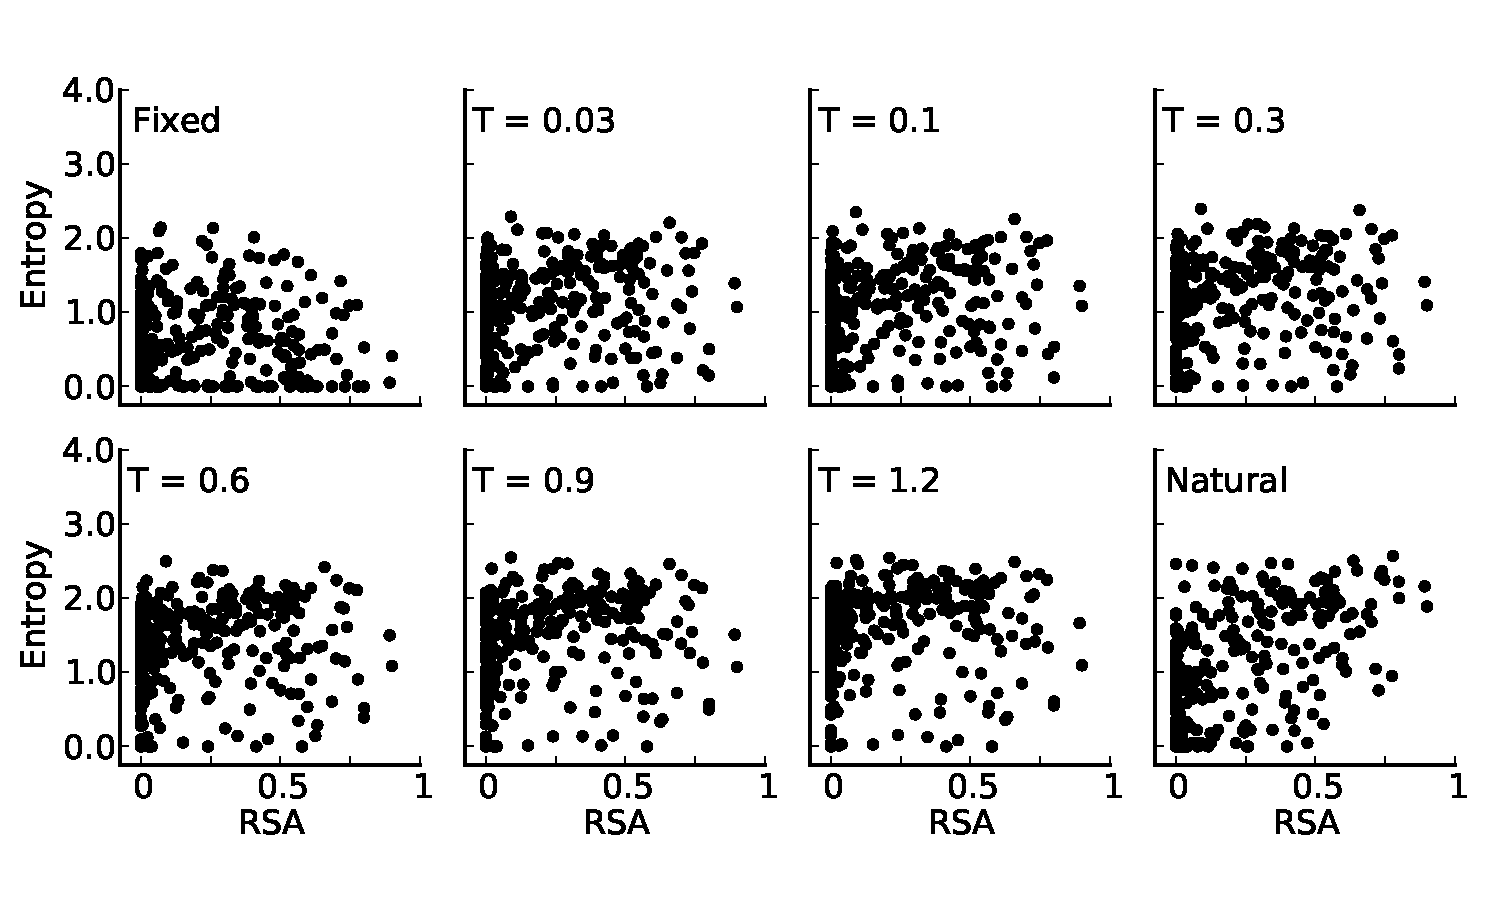
\includegraphics[width = 6.5in]{figures/RSA_vs_Entropy_1PV1_Combination_Plot.pdf}}

\noindent Figure S3. Site entropy versus Relative Solvent Accessibility (RSA) for designed and natural sequence alignments of the protein S-formylglutathione hydrolase (PDB: 1PV1, chain A). {\color{blue}\emph{[Methods?$\rightarrow$ ]} RSA values are calculated from the published PDB structure.} Natural sequences exhibit a clear trend of higher site variability at higher RSA values. The flexible backbone designs exhibit a similar trend but the fixed backbone designs do not.
\customlabel{Entropy_vs_RSA_example}{S3}

\newpage

\centerline{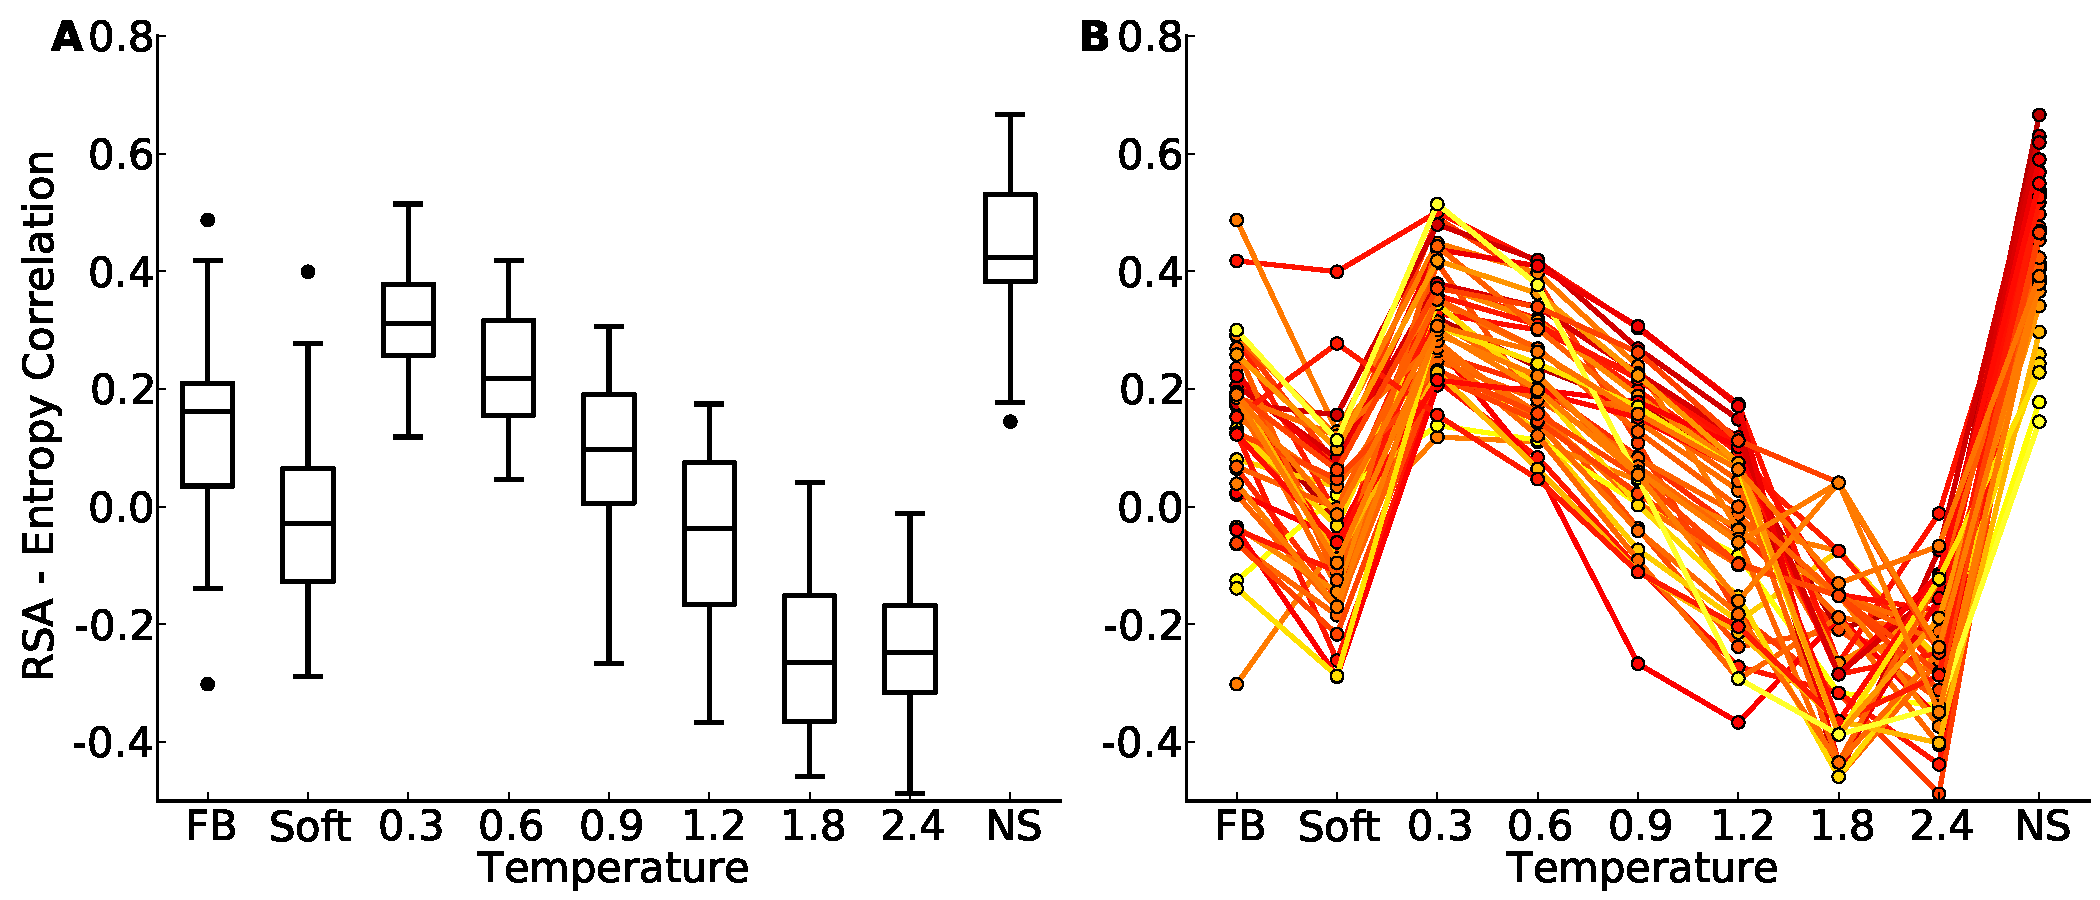
\includegraphics[width = 6in]{figures/Cor_Mean_Entropy_RSA_Combination_Plot_Noah.pdf}}
\noindent Figure S4. Distributions of correlation coefficients between site entropy and RSA, for the yeast-proteins data set. ``FB'' indicates fixed-backbone design, ``Soft'' indicates soft backbone design, and ``NS'' indicates natural sequences. (A) Distributions represented as boxplots. (B) Correlation coefficients for individual proteins. Lines connect identical structures in the different design conditions. The color shading represents the strength of the correlation for the natural sequence alignment. In general, natural proteins display a stronger correlation between site entropy and RSA than designed proteins.

\customlabel{Correlation_figure_Noah}{S4}




\end{document}